\documentclass[a4paper]{book}
\usepackage{makeidx}
\usepackage{graphicx}
\usepackage{multicol}
\usepackage{float}
\usepackage{listings}
\usepackage{color}
\usepackage{ifthen}
\usepackage[table]{xcolor}
\usepackage{textcomp}
\usepackage{alltt}
\usepackage{ifpdf}
\ifpdf
\usepackage[pdftex,
            pagebackref=true,
            colorlinks=true,
            linkcolor=blue,
            unicode
           ]{hyperref}
\else
\usepackage[ps2pdf,
            pagebackref=true,
            colorlinks=true,
            linkcolor=blue,
            unicode
           ]{hyperref}
\usepackage{pspicture}
\fi
\usepackage[utf8]{inputenc}
\usepackage{mathptmx}
\usepackage[scaled=.90]{helvet}
\usepackage{courier}
\usepackage{doxygen}
\lstset{language=C++,inputencoding=utf8,basicstyle=\footnotesize,breaklines=true,breakatwhitespace=true,tabsize=8,numbers=left }
\makeindex
\setcounter{tocdepth}{3}
\renewcommand{\footrulewidth}{0.4pt}
\begin{document}
\hypersetup{pageanchor=false}
\begin{titlepage}
\vspace*{7cm}
\begin{center}
{\Large JUMPUserInterface \\[1ex]\large 1.0 }\\
\vspace*{1cm}
{\large Generated by Doxygen 1.7.3}\\
\vspace*{0.5cm}
{\small Sun Mar 13 2011 16:47:29}\\
\end{center}
\end{titlepage}
\clearemptydoublepage
\pagenumbering{roman}
\tableofcontents
\clearemptydoublepage
\pagenumbering{arabic}
\hypersetup{pageanchor=true}
\chapter{JUMP User Interface Module Programming Guide}
\label{index}\hypertarget{index}{}{\bfseries JUMP Database Module} is an collection of classes that are wrappers and facades around the \href{http://developer.apple.com/library/mac/#documentation/cocoa/conceptual/CoreData/cdProgrammingGuide.html}{\tt Apple Core Data Framework}.\par
 \par
 You should have at least an basic experiencie with this powerful Apple framework to fully understand this module, he doesn't abstract or replace the Core Data, it just make your life more easy.\par
 \par
 The main component of this module are the \hyperlink{interface_j_p_d_b_manager}{Database Manager}. The manager center the main Core Data components in a single class and facilitate a collection of methods to perform main tasks around it. Also the manager could be used as a \hyperlink{interface_j_p_d_b_manager_singleton}{Singleton Instance} facilitating even more your database operations.

This diagram shows all components of the Database Manager operations and his components.\par
 \par
 

\subsection*{Learn more about this module in the following sections:}


\begin{DoxyItemize}
\item \hyperlink{basic_uses}{Basic Uses}
\item \hyperlink{errors}{Handling Errors}
\item \hyperlink{queries}{Performing Queries} 
\end{DoxyItemize}
\chapter{Working with colors}
\label{colors}
\hypertarget{colors}{}
\hyperlink{interface_j_p_color}{JPColor} is an Color Object that encapsulate information about colors on different color spaces. 

Is similar to the \href{http://developer.apple.com/library/ios/#documentation/uikit/reference/UIColor_Class/Reference/Reference.html}{\tt UIKit/UIColor class}, but with a lot of more convenient and powerfull features. Contains several convenient methods to easily create colors and convert between spaces.

\subsection*{Creating colors }

An example to how to create an \hyperlink{interface_j_p_color}{JPColor} with RGB values. 
\begin{DoxyCode}
 JPColor anColor = [JPColor initWithRed:255 G:0 B:0 opacity:100];
\end{DoxyCode}
 The above code create an {\bfseries red} color. Note that \hyperlink{interface_j_p_color}{JPColor} use an Photoshop-\/like values (0-\/255) to represent RGB colors. So once created an \hyperlink{interface_j_p_color}{JPColor} is easy to convert it to an UIColor like this: 
\begin{DoxyCode}
 UIColor anUIColor = [[JPColor initWithRed:255 G:0 B:0 opacity:100] UIColor];
\end{DoxyCode}
 You also can create color using different color spaces, like CMYK; 
\begin{DoxyCode}
 JPColor *cmyk = [JPColor initWithCyan:0 M:100 Y:100: K:0 opacity:100];
\end{DoxyCode}
 Or an CSS string, like this: 
\begin{DoxyCode}
 JPColor *color = [JPColor initWithCSS:@"#2658e8"];
\end{DoxyCode}


\subsection*{Colors Templates}

\hyperlink{interface_j_p_color}{JPColor} includes an collection of color templates methods that follow the \href{http://www.w3.org/TR/css3-color/#svg-color}{\tt W3C CSS 3 Extended Colors Keywords}. You can retrieve this methods simply calling his name, like this: 
\begin{DoxyCode}
 JPColor *seaGreenColor = [JPColor seagreen];
\end{DoxyCode}


\subsection*{Colors Type Structures}

\hyperlink{interface_j_p_color}{JPColor} return different \hyperlink{_j_p_color_types_8h}{structures types} with values for different color spaces. See \hyperlink{interface_j_p_color_a659b3f9caaf643fc6e9643b8470014f6}{RGB}, \hyperlink{interface_j_p_color_a06d575f03ff1692f65871d0485b62ae6}{CMYK} and \hyperlink{interface_j_p_color_a00bf425621fe08bd7eb6154be6b5a8a9}{HSV} properties to learn more about it. Here one exampe retrieving an CMYK structure and displaying it: 
\begin{DoxyCode}
 JPColor *anColor = [JPColor greenColor];
 JPcmyk repr = [anColor CMYK];
 
 // Print values.
 NSLog( @"C:%i, M:%i, Y:%i, K:%i", repr.C, repr.M, repr.Y, repr.K );
\end{DoxyCode}
  
\chapter{Class Index}
\section{Class List}
Here are the classes, structs, unions and interfaces with brief descriptions:\begin{DoxyCompactList}
\item\contentsline{section}{\hyperlink{interface_j_p_d_b_manager}{JPDBManager} (Database Manager are one Facade around {\bfseries Core Data} classes that facilitate the main operations around the {\bfseries Core Data Framework{\bfseries  }})}{\pageref{interface_j_p_d_b_manager}}{}
\item\contentsline{section}{\hyperlink{interface_j_p_d_b_manager_action}{JPDBManagerAction} ({\bfseries Database Manager Action} pack all data and settings to perform some database operation )}{\pageref{interface_j_p_d_b_manager_action}}{}
\item\contentsline{section}{\hyperlink{interface_j_p_d_b_manager_singleton}{JPDBManagerSingleton} (Singleton instance of \hyperlink{interface_j_p_d_b_manager}{Database Manager} that handle the {\bfseries Core Data Environment} )}{\pageref{interface_j_p_d_b_manager_singleton}}{}
\end{DoxyCompactList}

\chapter{File Index}
\section{File List}
Here is a list of all documented files with brief descriptions:\begin{DoxyCompactList}
\item\contentsline{section}{/Users/Paulo/Projects/JUMP/JUMPUserInterface/Headers/{\bfseries JPColor.h} }{\pageref{_j_p_color_8h}}{}
\item\contentsline{section}{/Users/Paulo/Projects/JUMP/JUMPUserInterface/Headers/\hyperlink{_j_p_color_convert_functions_8h}{JPColorConvertFunctions.h} (\hyperlink{interface_j_p_color}{JPColor} functions to convert between color spaces )}{\pageref{_j_p_color_convert_functions_8h}}{}
\item\contentsline{section}{/Users/Paulo/Projects/JUMP/JUMPUserInterface/Headers/\hyperlink{_j_p_color_functions_8h}{JPColorFunctions.h} (\hyperlink{interface_j_p_color}{JPColor} utility and helper functions )}{\pageref{_j_p_color_functions_8h}}{}
\item\contentsline{section}{/Users/Paulo/Projects/JUMP/JUMPUserInterface/Headers/{\bfseries JPColorTemplates.h} }{\pageref{_j_p_color_templates_8h}}{}
\item\contentsline{section}{/Users/Paulo/Projects/JUMP/JUMPUserInterface/Headers/\hyperlink{_j_p_color_types_8h}{JPColorTypes.h} (\hyperlink{interface_j_p_color}{JPColor} Data Type Structure for different color spaces )}{\pageref{_j_p_color_types_8h}}{}
\item\contentsline{section}{/Users/Paulo/Projects/JUMP/JUMPUserInterface/Headers/{\bfseries JUMPUserInterface.h} }{\pageref{_j_u_m_p_user_interface_8h}}{}
\end{DoxyCompactList}

\chapter{Class Documentation}
\hypertarget{struct_j_pcmy}{
\section{JPcmy Struct Reference}
\label{struct_j_pcmy}\index{JPcmy@{JPcmy}}
}


\hyperlink{interface_j_p_color}{JPColor} CMY Structure Type.  




{\ttfamily \#include $<$JPColorTypes.h$>$}

\subsection*{Public Attributes}
\begin{DoxyCompactItemize}
\item 
int \hyperlink{struct_j_pcmy_acb02d8f855f9f095cb4f124780184d70}{C}
\item 
int \hyperlink{struct_j_pcmy_ac6483cc803718dbcfd99ce13bc380923}{M}
\item 
int \hyperlink{struct_j_pcmy_aa06e890397d56b7d4e8bb64aa1e82b7c}{Y}
\end{DoxyCompactItemize}


\subsection{Detailed Description}
\hyperlink{interface_j_p_color}{JPColor} CMY Structure Type. 

\subsection{Member Data Documentation}
\hypertarget{struct_j_pcmy_acb02d8f855f9f095cb4f124780184d70}{
\index{JPcmy@{JPcmy}!C@{C}}
\index{C@{C}!JPcmy@{JPcmy}}
\subsubsection[{C}]{\setlength{\rightskip}{0pt plus 5cm}int {\bf JPcmy::C}}}
\label{struct_j_pcmy_acb02d8f855f9f095cb4f124780184d70}
Cyan (0-\/100) value \hypertarget{struct_j_pcmy_ac6483cc803718dbcfd99ce13bc380923}{
\index{JPcmy@{JPcmy}!M@{M}}
\index{M@{M}!JPcmy@{JPcmy}}
\subsubsection[{M}]{\setlength{\rightskip}{0pt plus 5cm}int {\bf JPcmy::M}}}
\label{struct_j_pcmy_ac6483cc803718dbcfd99ce13bc380923}
Magenta (0-\/100) value \hypertarget{struct_j_pcmy_aa06e890397d56b7d4e8bb64aa1e82b7c}{
\index{JPcmy@{JPcmy}!Y@{Y}}
\index{Y@{Y}!JPcmy@{JPcmy}}
\subsubsection[{Y}]{\setlength{\rightskip}{0pt plus 5cm}int {\bf JPcmy::Y}}}
\label{struct_j_pcmy_aa06e890397d56b7d4e8bb64aa1e82b7c}
Yellow (0-\/100) value 

The documentation for this struct was generated from the following file:\begin{DoxyCompactItemize}
\item 
/Users/Paulo/Projects/JUMP/JUMPUserInterface/Headers/\hyperlink{_j_p_color_types_8h}{JPColorTypes.h}\end{DoxyCompactItemize}

\hypertarget{struct_j_pcmyk}{
\section{JPcmyk Struct Reference}
\label{struct_j_pcmyk}\index{JPcmyk@{JPcmyk}}
}


\hyperlink{interface_j_p_color}{JPColor} CMYK Structure Type.  




{\ttfamily \#include $<$JPColorTypes.h$>$}

\subsection*{Public Attributes}
\begin{DoxyCompactItemize}
\item 
int \hyperlink{struct_j_pcmyk_a31b198bd6e353092dc4ca5fd489baf29}{C}
\item 
int \hyperlink{struct_j_pcmyk_a90de4545615a3622b5ea4f83d3ca3479}{M}
\item 
int \hyperlink{struct_j_pcmyk_a54bb8ef1c6b8d49f5aed98f5ad9e3053}{Y}
\item 
int \hyperlink{struct_j_pcmyk_aaae615286949bac30609a3a29a20e5fb}{K}
\end{DoxyCompactItemize}


\subsection{Detailed Description}
\hyperlink{interface_j_p_color}{JPColor} CMYK Structure Type. Use \hyperlink{_j_p_color_functions_8h_ace4eb5bbf6392366d0cc6ae57313d6d8}{JPCreateCMYKType} to conveniently create this structure. \begin{DoxySeeAlso}{See also}
\hyperlink{_j_p_color_convert_functions_8h_a8c9831bc0a46f817ca27293ee2c3136d}{JPConvertRGBtoCMYK}, \hyperlink{_j_p_color_convert_functions_8h_afbace75877e5f8a1e13cd3cd6862d5dc}{JPConvertCMYKtoRGB} functions. 
\end{DoxySeeAlso}


\subsection{Member Data Documentation}
\hypertarget{struct_j_pcmyk_a31b198bd6e353092dc4ca5fd489baf29}{
\index{JPcmyk@{JPcmyk}!C@{C}}
\index{C@{C}!JPcmyk@{JPcmyk}}
\subsubsection[{C}]{\setlength{\rightskip}{0pt plus 5cm}int {\bf JPcmyk::C}}}
\label{struct_j_pcmyk_a31b198bd6e353092dc4ca5fd489baf29}
Cyan (0-\/100) value \hypertarget{struct_j_pcmyk_a90de4545615a3622b5ea4f83d3ca3479}{
\index{JPcmyk@{JPcmyk}!M@{M}}
\index{M@{M}!JPcmyk@{JPcmyk}}
\subsubsection[{M}]{\setlength{\rightskip}{0pt plus 5cm}int {\bf JPcmyk::M}}}
\label{struct_j_pcmyk_a90de4545615a3622b5ea4f83d3ca3479}
Magenta (0-\/100) value \hypertarget{struct_j_pcmyk_a54bb8ef1c6b8d49f5aed98f5ad9e3053}{
\index{JPcmyk@{JPcmyk}!Y@{Y}}
\index{Y@{Y}!JPcmyk@{JPcmyk}}
\subsubsection[{Y}]{\setlength{\rightskip}{0pt plus 5cm}int {\bf JPcmyk::Y}}}
\label{struct_j_pcmyk_a54bb8ef1c6b8d49f5aed98f5ad9e3053}
Yellow (0-\/100) value \hypertarget{struct_j_pcmyk_aaae615286949bac30609a3a29a20e5fb}{
\index{JPcmyk@{JPcmyk}!K@{K}}
\index{K@{K}!JPcmyk@{JPcmyk}}
\subsubsection[{K}]{\setlength{\rightskip}{0pt plus 5cm}int {\bf JPcmyk::K}}}
\label{struct_j_pcmyk_aaae615286949bac30609a3a29a20e5fb}
Black (0-\/100) value 

The documentation for this struct was generated from the following file:\begin{DoxyCompactItemize}
\item 
/Users/Paulo/Projects/JUMP/JUMPUserInterface/Headers/\hyperlink{_j_p_color_types_8h}{JPColorTypes.h}\end{DoxyCompactItemize}

\hypertarget{interface_j_p_color}{
\section{JPColor Class Reference}
\label{interface_j_p_color}\index{JPColor@{JPColor}}
}


\hyperlink{interface_j_p_color}{JPColor} is an Color Object that encapsulate information about colors on different color spaces.  




{\ttfamily \#import $<$JPColor.h$>$}

\subsection*{Properties}
\begin{DoxyCompactItemize}
\item 
\hypertarget{interface_j_p_color_a5f08f4731c881872d34b7e18546bedb3}{
int \hyperlink{interface_j_p_color_a5f08f4731c881872d34b7e18546bedb3}{R}}
\label{interface_j_p_color_a5f08f4731c881872d34b7e18546bedb3}

\begin{DoxyCompactList}\small\item\em Red value (0-\/255) \item\end{DoxyCompactList}\item 
\hypertarget{interface_j_p_color_a6b7861ca88763bb2baef53e3afc04e32}{
int \hyperlink{interface_j_p_color_a6b7861ca88763bb2baef53e3afc04e32}{G}}
\label{interface_j_p_color_a6b7861ca88763bb2baef53e3afc04e32}

\begin{DoxyCompactList}\small\item\em Green value (0-\/255) \item\end{DoxyCompactList}\item 
\hypertarget{interface_j_p_color_a1e438555e86971a216f05bd8b4873d4a}{
int \hyperlink{interface_j_p_color_a1e438555e86971a216f05bd8b4873d4a}{B}}
\label{interface_j_p_color_a1e438555e86971a216f05bd8b4873d4a}

\begin{DoxyCompactList}\small\item\em Blue value (0-\/255) \item\end{DoxyCompactList}\item 
\hypertarget{interface_j_p_color_a0fce04992ae5d5c4e90468f7dd9717f2}{
float \hyperlink{interface_j_p_color_a0fce04992ae5d5c4e90468f7dd9717f2}{opacity}}
\label{interface_j_p_color_a0fce04992ae5d5c4e90468f7dd9717f2}

\begin{DoxyCompactList}\small\item\em opacity value (0-\/100) \item\end{DoxyCompactList}\item 
\hypertarget{interface_j_p_color_a659b3f9caaf643fc6e9643b8470014f6}{
\hyperlink{struct_j_prgb}{JPrgb} \hyperlink{interface_j_p_color_a659b3f9caaf643fc6e9643b8470014f6}{RGB}}
\label{interface_j_p_color_a659b3f9caaf643fc6e9643b8470014f6}

\begin{DoxyCompactList}\small\item\em An \hyperlink{struct_j_prgb}{JPrgb} type with setted Red, Green and Blue representation of this object. \item\end{DoxyCompactList}\item 
\hypertarget{interface_j_p_color_a06d575f03ff1692f65871d0485b62ae6}{
\hyperlink{struct_j_pcmyk}{JPcmyk} \hyperlink{interface_j_p_color_a06d575f03ff1692f65871d0485b62ae6}{CMYK}}
\label{interface_j_p_color_a06d575f03ff1692f65871d0485b62ae6}

\begin{DoxyCompactList}\small\item\em An \hyperlink{struct_j_pcmyk}{JPcmyk} type with setted Cyan, Magenta, Yellow and Black representation of this object. \item\end{DoxyCompactList}\item 
\hypertarget{interface_j_p_color_a00bf425621fe08bd7eb6154be6b5a8a9}{
\hyperlink{struct_j_phsv}{JPhsv} \hyperlink{interface_j_p_color_a00bf425621fe08bd7eb6154be6b5a8a9}{HSV}}
\label{interface_j_p_color_a00bf425621fe08bd7eb6154be6b5a8a9}

\begin{DoxyCompactList}\small\item\em An \hyperlink{struct_j_phsv}{JPhsv} type with setted Hue, Saturation and Brightness representation of this object. \item\end{DoxyCompactList}\item 
\hypertarget{interface_j_p_color_aa1fe8baa6f05c753211a016c18a86ce5}{
CGBlendMode \hyperlink{interface_j_p_color_aa1fe8baa6f05c753211a016c18a86ce5}{blendMode}}
\label{interface_j_p_color_aa1fe8baa6f05c753211a016c18a86ce5}

\begin{DoxyCompactList}\small\item\em An Quartz Blend Mode associated with this color. \item\end{DoxyCompactList}\item 
CGColorRef \hyperlink{interface_j_p_color_a6b74a8281b3ebf94eeda2db00ab048fb}{CGColor}
\begin{DoxyCompactList}\small\item\em The Quartz Color reference that corresponds to the receiver’s color. \item\end{DoxyCompactList}\item 
\hypertarget{interface_j_p_color_aa2114c2e3a1064060f461a30c04e9368}{
UIColor $\ast$ \hyperlink{interface_j_p_color_aa2114c2e3a1064060f461a30c04e9368}{UIColor}}
\label{interface_j_p_color_aa2114c2e3a1064060f461a30c04e9368}

\begin{DoxyCompactList}\small\item\em Generate an UIColor object with stored values os this object. \item\end{DoxyCompactList}\end{DoxyCompactItemize}
\subsection*{Init Methods}
\begin{DoxyCompactItemize}
\item 
(\hyperlink{interface_j_p_color}{JPColor} $\ast$) + \hyperlink{interface_j_p_color_a5f07346b927b9b7355dc51b1330641f3}{initWithDictionary:}
\begin{DoxyCompactList}\small\item\em Initializes and returns an \hyperlink{interface_j_p_color}{JPColor} from a NSDictionary. \item\end{DoxyCompactList}\item 
(\hyperlink{interface_j_p_color}{JPColor} $\ast$) + \hyperlink{interface_j_p_color_a0e5015082d770f62b9778da3d00e1503}{initWithGrayScale:opacity:}
\begin{DoxyCompactList}\small\item\em Initializes and returns an \hyperlink{interface_j_p_color}{JPColor} using the specified opacity and grayscale values. \item\end{DoxyCompactList}\item 
(\hyperlink{interface_j_p_color}{JPColor} $\ast$) + \hyperlink{interface_j_p_color_a825ecad2dbb5a12d86e07263ecde4e27}{initWithRed:G:B:opacity:}
\begin{DoxyCompactList}\small\item\em Initializes and returns a \hyperlink{interface_j_p_color}{JPColor} object using the specified opacity and RGB component values. \item\end{DoxyCompactList}\item 
(\hyperlink{interface_j_p_color}{JPColor} $\ast$) + \hyperlink{interface_j_p_color_a608d8aae9deb9db4549eaaa0cdb05604}{initWithHue:S:V:opacity:}
\begin{DoxyCompactList}\small\item\em Initializes and returns a \hyperlink{interface_j_p_color}{JPColor} object using the specified opacity and HSB color space component values. \item\end{DoxyCompactList}\item 
(\hyperlink{interface_j_p_color}{JPColor} $\ast$) + \hyperlink{interface_j_p_color_ade815fda8c301fe43cda27b0f5312c9b}{initWithCyan:M:Y:K:opacity:}
\begin{DoxyCompactList}\small\item\em Initializes and returns a \hyperlink{interface_j_p_color}{JPColor} object using the specified opacity and CMYK color space component values. \item\end{DoxyCompactList}\item 
(\hyperlink{interface_j_p_color}{JPColor} $\ast$) + \hyperlink{interface_j_p_color_a244c1758fdf57f4beb62a5884d5ad142}{initWithJPrgb:}
\begin{DoxyCompactList}\small\item\em Initializes and returns a \hyperlink{interface_j_p_color}{JPColor} object using an \hyperlink{struct_j_prgb}{JPrgb} type. \item\end{DoxyCompactList}\item 
(\hyperlink{interface_j_p_color}{JPColor} $\ast$) + \hyperlink{interface_j_p_color_a8cc0f1ebfd272fca56fbcc1e333c0cc1}{iniWithJPrgb:opacity:}
\begin{DoxyCompactList}\small\item\em Initializes and returns a \hyperlink{interface_j_p_color}{JPColor} object using an \hyperlink{struct_j_prgb}{JPrgb} type and opacity. \item\end{DoxyCompactList}\item 
(\hyperlink{interface_j_p_color}{JPColor} $\ast$) + \hyperlink{interface_j_p_color_a2a76a3cee7b52f969f29edd021fe66ee}{initWithCSS:}
\begin{DoxyCompactList}\small\item\em Initializes and returns a \hyperlink{interface_j_p_color}{JPColor} object using an String representing an CSS color. \item\end{DoxyCompactList}\item 
(\hyperlink{interface_j_p_color}{JPColor} $\ast$) + \hyperlink{interface_j_p_color_ae76fd408d66035ae1ccfe1fb8820e852}{initWithRed:G:B:opacity:blendMode:}
\begin{DoxyCompactList}\small\item\em Initializes and returns a \hyperlink{interface_j_p_color}{JPColor} object using the specified opacity and RGB component values. \item\end{DoxyCompactList}\end{DoxyCompactItemize}
\subsection*{Convert Methods}
\begin{DoxyCompactItemize}
\item 
(NSDictionary $\ast$) -\/ \hyperlink{interface_j_p_color_a4e9484ec16fc8b0fa4dcf51d705e1dc2}{dictionary}
\begin{DoxyCompactList}\small\item\em Parse the stored values of this object to an NSDictionary. \item\end{DoxyCompactList}\end{DoxyCompactItemize}
\subsection*{Set Methods}
\begin{DoxyCompactItemize}
\item 
(void) -\/ \hyperlink{interface_j_p_color_a0a99e0e61f21bb33cc7e4342d7ab950d}{setColorRed:G:B:opacity:}
\begin{DoxyCompactList}\small\item\em Set Red, Green, Blue and opacity values. \item\end{DoxyCompactList}\item 
(void) -\/ \hyperlink{interface_j_p_color_aead8ca7007e2ed10f75f569bc8d652fb}{setColorRed:G:B:opacity:blendMode:}
\begin{DoxyCompactList}\small\item\em Set Red, Green, Blue, opacity and Blend Effect values. \item\end{DoxyCompactList}\item 
(void) -\/ \hyperlink{interface_j_p_color_ab2b12824d02c5203ac44dcd9784c4008}{setColorWithHue:S:V:opacity:}
\begin{DoxyCompactList}\small\item\em Set Hue, Saturaton, Brigtness and opacity. \item\end{DoxyCompactList}\item 
(void) -\/ \hyperlink{interface_j_p_color_adbab2d8cf2734971130ccbf9feda9d1a}{setColorWithCSS:}
\begin{DoxyCompactList}\small\item\em Set color with an String representing an CSS color. \item\end{DoxyCompactList}\item 
(void) -\/ \hyperlink{interface_j_p_color_acb1f82a97662b72baaf316ff6f9eb4bb}{setColorWithDictionary:}
\begin{DoxyCompactList}\small\item\em Set color with an NSDictionary. \item\end{DoxyCompactList}\end{DoxyCompactItemize}
\subsection*{Color Processing Methods}
\begin{DoxyCompactItemize}
\item 
(\hyperlink{interface_j_p_color}{JPColor} $\ast$) -\/ \hyperlink{interface_j_p_color_a32498959b299b8fbf19c39c00991df60}{multiplyHue:saturation:value:}
\begin{DoxyCompactList}\small\item\em Multiply new HSV values to current object. \item\end{DoxyCompactList}\item 
(\hyperlink{interface_j_p_color}{JPColor} $\ast$) -\/ \hyperlink{interface_j_p_color_a6e09c9e02bc6036074e401e28c14bb57}{addHue:saturation:value:}
\begin{DoxyCompactList}\small\item\em Add new HSV values to current object. \item\end{DoxyCompactList}\item 
(\hyperlink{interface_j_p_color}{JPColor} $\ast$) -\/ \hyperlink{interface_j_p_color_a6ca5307a9f9e8ceb4dd1cd657cf90e25}{lighter}
\begin{DoxyCompactList}\small\item\em Add more light to current color. \item\end{DoxyCompactList}\item 
(\hyperlink{interface_j_p_color}{JPColor} $\ast$) -\/ \hyperlink{interface_j_p_color_ac5769a3a901b96c011d7a33bf54d0fb9}{darker}
\begin{DoxyCompactList}\small\item\em Remove light from current color (More darker). \item\end{DoxyCompactList}\item 
(\hyperlink{interface_j_p_color}{JPColor} $\ast$) -\/ \hyperlink{interface_j_p_color_a3e411517eae8c3d78d567b33a0888160}{copyWithAlpha:}
\begin{DoxyCompactList}\small\item\em Make a new copy of this object assigning one new opacity Value. \item\end{DoxyCompactList}\end{DoxyCompactItemize}
\subsection*{Color template methods}
\label{_amgrp7b749c2d171ff4698bb077b5c75d4638}
This methods retrieve color templates that follow the \href{http://www.w3.org/TR/css3-color/#svg-color}{\tt W3C CSS 3 Extended Colors Keywords. }. \begin{DoxyCompactItemize}
\item 
\hypertarget{interface_j_p_color_af66a1ea8ebef3b3378b22f0919c12d9c}{
(\hyperlink{interface_j_p_color}{JPColor} $\ast$) + {\bfseries lightGray}}
\label{interface_j_p_color_af66a1ea8ebef3b3378b22f0919c12d9c}

\item 
\hypertarget{interface_j_p_color_addb9e08446fa5092ab0ae6914af70ea1}{
(\hyperlink{interface_j_p_color}{JPColor} $\ast$) + {\bfseries darkGray}}
\label{interface_j_p_color_addb9e08446fa5092ab0ae6914af70ea1}

\item 
\hypertarget{interface_j_p_color_af519c4d0b4a75b857d7c7d940f792f31}{
(\hyperlink{interface_j_p_color}{JPColor} $\ast$) + {\bfseries clearColor}}
\label{interface_j_p_color_af519c4d0b4a75b857d7c7d940f792f31}

\item 
\hypertarget{interface_j_p_color_a164e9e771536daa3b597b1acaf9b0c5d}{
(\hyperlink{interface_j_p_color}{JPColor} $\ast$) + {\bfseries fuschia}}
\label{interface_j_p_color_a164e9e771536daa3b597b1acaf9b0c5d}

\item 
\hypertarget{interface_j_p_color_adf28e4c9016e070cf4813e27c5f0443a}{
(\hyperlink{interface_j_p_color}{JPColor} $\ast$) + {\bfseries transparent}}
\label{interface_j_p_color_adf28e4c9016e070cf4813e27c5f0443a}

\item 
\hypertarget{interface_j_p_color_ae1170c84dbe6a1803b2ef52a218b933e}{
(\hyperlink{interface_j_p_color}{JPColor} $\ast$) + {\bfseries aliceblue}}
\label{interface_j_p_color_ae1170c84dbe6a1803b2ef52a218b933e}

\item 
\hypertarget{interface_j_p_color_a8d43ffe93957038e9a4fee0c6e4fe51a}{
(\hyperlink{interface_j_p_color}{JPColor} $\ast$) + {\bfseries antiquewhite}}
\label{interface_j_p_color_a8d43ffe93957038e9a4fee0c6e4fe51a}

\item 
\hypertarget{interface_j_p_color_a07cf8656cb4fd559544b15cb11334f0c}{
(\hyperlink{interface_j_p_color}{JPColor} $\ast$) + {\bfseries aqua}}
\label{interface_j_p_color_a07cf8656cb4fd559544b15cb11334f0c}

\item 
\hypertarget{interface_j_p_color_a2f7a83e6af19dbdcad0b20f3e141e155}{
(\hyperlink{interface_j_p_color}{JPColor} $\ast$) + {\bfseries aquamarine}}
\label{interface_j_p_color_a2f7a83e6af19dbdcad0b20f3e141e155}

\item 
\hypertarget{interface_j_p_color_a22db5d07d75b657449504d080fc03099}{
(\hyperlink{interface_j_p_color}{JPColor} $\ast$) + {\bfseries azure}}
\label{interface_j_p_color_a22db5d07d75b657449504d080fc03099}

\item 
\hypertarget{interface_j_p_color_a5e36b90d086806040bc91b91f46cd309}{
(\hyperlink{interface_j_p_color}{JPColor} $\ast$) + {\bfseries beige}}
\label{interface_j_p_color_a5e36b90d086806040bc91b91f46cd309}

\item 
\hypertarget{interface_j_p_color_a708653ba0e7fe120ecc36a42a83b90a6}{
(\hyperlink{interface_j_p_color}{JPColor} $\ast$) + {\bfseries bisque}}
\label{interface_j_p_color_a708653ba0e7fe120ecc36a42a83b90a6}

\item 
\hypertarget{interface_j_p_color_a39049ec6fabe676dfc499af68261388a}{
(\hyperlink{interface_j_p_color}{JPColor} $\ast$) + {\bfseries black}}
\label{interface_j_p_color_a39049ec6fabe676dfc499af68261388a}

\item 
\hypertarget{interface_j_p_color_af77e6b82c2d89f203e4fd35575ff06f4}{
(\hyperlink{interface_j_p_color}{JPColor} $\ast$) + {\bfseries blanchedalmond}}
\label{interface_j_p_color_af77e6b82c2d89f203e4fd35575ff06f4}

\item 
\hypertarget{interface_j_p_color_a6ec4ac9c03ca569937445f0f17ab69d2}{
(\hyperlink{interface_j_p_color}{JPColor} $\ast$) + {\bfseries blue}}
\label{interface_j_p_color_a6ec4ac9c03ca569937445f0f17ab69d2}

\item 
\hypertarget{interface_j_p_color_a86900b2359b21e4335e171d1c03f6e3d}{
(\hyperlink{interface_j_p_color}{JPColor} $\ast$) + {\bfseries blueviolet}}
\label{interface_j_p_color_a86900b2359b21e4335e171d1c03f6e3d}

\item 
\hypertarget{interface_j_p_color_a0a98869ac55cab1956f428620488e391}{
(\hyperlink{interface_j_p_color}{JPColor} $\ast$) + {\bfseries brown}}
\label{interface_j_p_color_a0a98869ac55cab1956f428620488e391}

\item 
\hypertarget{interface_j_p_color_a503e8feaba2214a597144a900fe8648c}{
(\hyperlink{interface_j_p_color}{JPColor} $\ast$) + {\bfseries burlywood}}
\label{interface_j_p_color_a503e8feaba2214a597144a900fe8648c}

\item 
\hypertarget{interface_j_p_color_a71048a73512776a829b08a33e1c359e6}{
(\hyperlink{interface_j_p_color}{JPColor} $\ast$) + {\bfseries cadetblue}}
\label{interface_j_p_color_a71048a73512776a829b08a33e1c359e6}

\item 
\hypertarget{interface_j_p_color_abb94831c97f9e81ce0ae185794e0773b}{
(\hyperlink{interface_j_p_color}{JPColor} $\ast$) + {\bfseries chartreuse}}
\label{interface_j_p_color_abb94831c97f9e81ce0ae185794e0773b}

\item 
\hypertarget{interface_j_p_color_ae9a0c221dca17792ffc9d7447a77b9c1}{
(\hyperlink{interface_j_p_color}{JPColor} $\ast$) + {\bfseries chocolate}}
\label{interface_j_p_color_ae9a0c221dca17792ffc9d7447a77b9c1}

\item 
\hypertarget{interface_j_p_color_ac4ed76798a561279b444c76a12eec60b}{
(\hyperlink{interface_j_p_color}{JPColor} $\ast$) + {\bfseries coral}}
\label{interface_j_p_color_ac4ed76798a561279b444c76a12eec60b}

\item 
\hypertarget{interface_j_p_color_a051f1bfa4f9cf0457bb5cfc064776609}{
(\hyperlink{interface_j_p_color}{JPColor} $\ast$) + {\bfseries cornflowerblue}}
\label{interface_j_p_color_a051f1bfa4f9cf0457bb5cfc064776609}

\item 
\hypertarget{interface_j_p_color_a69501e83c6d8b0429336dcef5811a9ae}{
(\hyperlink{interface_j_p_color}{JPColor} $\ast$) + {\bfseries cornsilk}}
\label{interface_j_p_color_a69501e83c6d8b0429336dcef5811a9ae}

\item 
\hypertarget{interface_j_p_color_a48112cf3d8ce2775d7877b66be5db827}{
(\hyperlink{interface_j_p_color}{JPColor} $\ast$) + {\bfseries crimson}}
\label{interface_j_p_color_a48112cf3d8ce2775d7877b66be5db827}

\item 
\hypertarget{interface_j_p_color_a3da6201287a0aac7326ad304dc5a6475}{
(\hyperlink{interface_j_p_color}{JPColor} $\ast$) + {\bfseries cyan}}
\label{interface_j_p_color_a3da6201287a0aac7326ad304dc5a6475}

\item 
\hypertarget{interface_j_p_color_a69fa2db1fa05b42cbe5881ffc5673ba9}{
(\hyperlink{interface_j_p_color}{JPColor} $\ast$) + {\bfseries darkblue}}
\label{interface_j_p_color_a69fa2db1fa05b42cbe5881ffc5673ba9}

\item 
\hypertarget{interface_j_p_color_a12995d729a9fc1676e9c8a0cea52fdbc}{
(\hyperlink{interface_j_p_color}{JPColor} $\ast$) + {\bfseries darkcyan}}
\label{interface_j_p_color_a12995d729a9fc1676e9c8a0cea52fdbc}

\item 
\hypertarget{interface_j_p_color_ad856f619f184ebbf7997fa397d432651}{
(\hyperlink{interface_j_p_color}{JPColor} $\ast$) + {\bfseries darkgoldenrod}}
\label{interface_j_p_color_ad856f619f184ebbf7997fa397d432651}

\item 
\hypertarget{interface_j_p_color_aee8b774fee2582a75014d3a3db91bcc0}{
(\hyperlink{interface_j_p_color}{JPColor} $\ast$) + {\bfseries darkgray}}
\label{interface_j_p_color_aee8b774fee2582a75014d3a3db91bcc0}

\item 
\hypertarget{interface_j_p_color_af8a473326f62b7832c6aef456c7cad5f}{
(\hyperlink{interface_j_p_color}{JPColor} $\ast$) + {\bfseries darkgreen}}
\label{interface_j_p_color_af8a473326f62b7832c6aef456c7cad5f}

\item 
\hypertarget{interface_j_p_color_acb3f9b5e4fcb5212be2b78fdfaaa5e34}{
(\hyperlink{interface_j_p_color}{JPColor} $\ast$) + {\bfseries darkgrey}}
\label{interface_j_p_color_acb3f9b5e4fcb5212be2b78fdfaaa5e34}

\item 
\hypertarget{interface_j_p_color_a38fa47830ea0803042b381bd91e18f02}{
(\hyperlink{interface_j_p_color}{JPColor} $\ast$) + {\bfseries darkkhaki}}
\label{interface_j_p_color_a38fa47830ea0803042b381bd91e18f02}

\item 
\hypertarget{interface_j_p_color_a05e1d1aafa1cda22ef2b6ea3848208e2}{
(\hyperlink{interface_j_p_color}{JPColor} $\ast$) + {\bfseries darkmagenta}}
\label{interface_j_p_color_a05e1d1aafa1cda22ef2b6ea3848208e2}

\item 
\hypertarget{interface_j_p_color_a366422ec3e3ece29901504521103da94}{
(\hyperlink{interface_j_p_color}{JPColor} $\ast$) + {\bfseries darkolivegreen}}
\label{interface_j_p_color_a366422ec3e3ece29901504521103da94}

\item 
\hypertarget{interface_j_p_color_adceb3e2fa05be9a0eafa78d448406af6}{
(\hyperlink{interface_j_p_color}{JPColor} $\ast$) + {\bfseries darkorange}}
\label{interface_j_p_color_adceb3e2fa05be9a0eafa78d448406af6}

\item 
\hypertarget{interface_j_p_color_afd854343ba8522151a9bbaea3b515d50}{
(\hyperlink{interface_j_p_color}{JPColor} $\ast$) + {\bfseries darkorchid}}
\label{interface_j_p_color_afd854343ba8522151a9bbaea3b515d50}

\item 
\hypertarget{interface_j_p_color_a8b6591b6030e81d62051aba364914416}{
(\hyperlink{interface_j_p_color}{JPColor} $\ast$) + {\bfseries darkred}}
\label{interface_j_p_color_a8b6591b6030e81d62051aba364914416}

\item 
\hypertarget{interface_j_p_color_a97ba4dace0aacf72e6001307e771ab61}{
(\hyperlink{interface_j_p_color}{JPColor} $\ast$) + {\bfseries darksalmon}}
\label{interface_j_p_color_a97ba4dace0aacf72e6001307e771ab61}

\item 
\hypertarget{interface_j_p_color_ab39192018abad355f45f7ba624689efe}{
(\hyperlink{interface_j_p_color}{JPColor} $\ast$) + {\bfseries darkseagreen}}
\label{interface_j_p_color_ab39192018abad355f45f7ba624689efe}

\item 
\hypertarget{interface_j_p_color_aebaf6e5fe3be124ae138da4ae27e5a18}{
(\hyperlink{interface_j_p_color}{JPColor} $\ast$) + {\bfseries darkslateblue}}
\label{interface_j_p_color_aebaf6e5fe3be124ae138da4ae27e5a18}

\item 
\hypertarget{interface_j_p_color_a0a62d7fdc09b6aa8ae77de52e2523a11}{
(\hyperlink{interface_j_p_color}{JPColor} $\ast$) + {\bfseries darkslategray}}
\label{interface_j_p_color_a0a62d7fdc09b6aa8ae77de52e2523a11}

\item 
\hypertarget{interface_j_p_color_a253c1b1fed2c2046495372609305dccc}{
(\hyperlink{interface_j_p_color}{JPColor} $\ast$) + {\bfseries darkslategrey}}
\label{interface_j_p_color_a253c1b1fed2c2046495372609305dccc}

\item 
\hypertarget{interface_j_p_color_a9009bad971652fcbeb4a913b0a90a9bd}{
(\hyperlink{interface_j_p_color}{JPColor} $\ast$) + {\bfseries darkturquoise}}
\label{interface_j_p_color_a9009bad971652fcbeb4a913b0a90a9bd}

\item 
\hypertarget{interface_j_p_color_a081b059839af62f33110461f7032c688}{
(\hyperlink{interface_j_p_color}{JPColor} $\ast$) + {\bfseries darkviolet}}
\label{interface_j_p_color_a081b059839af62f33110461f7032c688}

\item 
\hypertarget{interface_j_p_color_a30b2da6be3b63f2f6552c69bf35765db}{
(\hyperlink{interface_j_p_color}{JPColor} $\ast$) + {\bfseries deeppink}}
\label{interface_j_p_color_a30b2da6be3b63f2f6552c69bf35765db}

\item 
\hypertarget{interface_j_p_color_af6c1671ec3b6811746b5edccd5337fdc}{
(\hyperlink{interface_j_p_color}{JPColor} $\ast$) + {\bfseries deepskyblue}}
\label{interface_j_p_color_af6c1671ec3b6811746b5edccd5337fdc}

\item 
\hypertarget{interface_j_p_color_a02ffffbbbd59d7209c534ca51ea6d1a3}{
(\hyperlink{interface_j_p_color}{JPColor} $\ast$) + {\bfseries dimgray}}
\label{interface_j_p_color_a02ffffbbbd59d7209c534ca51ea6d1a3}

\item 
\hypertarget{interface_j_p_color_afda85cbfe80620877a404b1d90f6d29d}{
(\hyperlink{interface_j_p_color}{JPColor} $\ast$) + {\bfseries dimgrey}}
\label{interface_j_p_color_afda85cbfe80620877a404b1d90f6d29d}

\item 
\hypertarget{interface_j_p_color_ad959b1cce02e085184ad5097dcb0f0ce}{
(\hyperlink{interface_j_p_color}{JPColor} $\ast$) + {\bfseries dodgerblue}}
\label{interface_j_p_color_ad959b1cce02e085184ad5097dcb0f0ce}

\item 
\hypertarget{interface_j_p_color_ae1ed6c3cbd32d04856ba74fc56a8063b}{
(\hyperlink{interface_j_p_color}{JPColor} $\ast$) + {\bfseries firebrick}}
\label{interface_j_p_color_ae1ed6c3cbd32d04856ba74fc56a8063b}

\item 
\hypertarget{interface_j_p_color_a8bffe7b0fcdf83a87ae1c2a0f3a186ed}{
(\hyperlink{interface_j_p_color}{JPColor} $\ast$) + {\bfseries floralwhite}}
\label{interface_j_p_color_a8bffe7b0fcdf83a87ae1c2a0f3a186ed}

\item 
\hypertarget{interface_j_p_color_a0384648257b3392c0e83686aef7a091e}{
(\hyperlink{interface_j_p_color}{JPColor} $\ast$) + {\bfseries forestgreen}}
\label{interface_j_p_color_a0384648257b3392c0e83686aef7a091e}

\item 
\hypertarget{interface_j_p_color_a04cdd3157ac626a3cdbb184fb70d8358}{
(\hyperlink{interface_j_p_color}{JPColor} $\ast$) + {\bfseries fuchsia}}
\label{interface_j_p_color_a04cdd3157ac626a3cdbb184fb70d8358}

\item 
\hypertarget{interface_j_p_color_a26ba58f343c7e190e6b647ae9e4ad2f0}{
(\hyperlink{interface_j_p_color}{JPColor} $\ast$) + {\bfseries gainsboro}}
\label{interface_j_p_color_a26ba58f343c7e190e6b647ae9e4ad2f0}

\item 
\hypertarget{interface_j_p_color_a47e74c169fd41c769059ce6faaac76bb}{
(\hyperlink{interface_j_p_color}{JPColor} $\ast$) + {\bfseries ghostwhite}}
\label{interface_j_p_color_a47e74c169fd41c769059ce6faaac76bb}

\item 
\hypertarget{interface_j_p_color_a6430c451c29755d7aee7004e26ea6c30}{
(\hyperlink{interface_j_p_color}{JPColor} $\ast$) + {\bfseries gold}}
\label{interface_j_p_color_a6430c451c29755d7aee7004e26ea6c30}

\item 
\hypertarget{interface_j_p_color_a28fce9831a9ace23e2bb4e6088c3ea32}{
(\hyperlink{interface_j_p_color}{JPColor} $\ast$) + {\bfseries goldenrod}}
\label{interface_j_p_color_a28fce9831a9ace23e2bb4e6088c3ea32}

\item 
\hypertarget{interface_j_p_color_a4420f1ac02c6ff80093a24a797c1fb06}{
(\hyperlink{interface_j_p_color}{JPColor} $\ast$) + {\bfseries gray}}
\label{interface_j_p_color_a4420f1ac02c6ff80093a24a797c1fb06}

\item 
\hypertarget{interface_j_p_color_a0aed95f1124e54ee65c4bc7e3f27b0d0}{
(\hyperlink{interface_j_p_color}{JPColor} $\ast$) + {\bfseries green}}
\label{interface_j_p_color_a0aed95f1124e54ee65c4bc7e3f27b0d0}

\item 
\hypertarget{interface_j_p_color_abf5dd9ad35f513a3e42345f528b1d69c}{
(\hyperlink{interface_j_p_color}{JPColor} $\ast$) + {\bfseries greenyellow}}
\label{interface_j_p_color_abf5dd9ad35f513a3e42345f528b1d69c}

\item 
\hypertarget{interface_j_p_color_a6952a2469467ecedd2137eeca8a38a9c}{
(\hyperlink{interface_j_p_color}{JPColor} $\ast$) + {\bfseries grey}}
\label{interface_j_p_color_a6952a2469467ecedd2137eeca8a38a9c}

\item 
\hypertarget{interface_j_p_color_afefad99104a6daca4734184ec155205b}{
(\hyperlink{interface_j_p_color}{JPColor} $\ast$) + {\bfseries honeydew}}
\label{interface_j_p_color_afefad99104a6daca4734184ec155205b}

\item 
\hypertarget{interface_j_p_color_ab351754ee591a4ac2957da8c42d09234}{
(\hyperlink{interface_j_p_color}{JPColor} $\ast$) + {\bfseries hotpink}}
\label{interface_j_p_color_ab351754ee591a4ac2957da8c42d09234}

\item 
\hypertarget{interface_j_p_color_ab32db7544addacd8ee6111d9508c1d82}{
(\hyperlink{interface_j_p_color}{JPColor} $\ast$) + {\bfseries indianred}}
\label{interface_j_p_color_ab32db7544addacd8ee6111d9508c1d82}

\item 
\hypertarget{interface_j_p_color_a8995e6dcdf53834b55ee8953217103ff}{
(\hyperlink{interface_j_p_color}{JPColor} $\ast$) + {\bfseries indigo}}
\label{interface_j_p_color_a8995e6dcdf53834b55ee8953217103ff}

\item 
\hypertarget{interface_j_p_color_a5895f6204e604f00f74a7741e443ba12}{
(\hyperlink{interface_j_p_color}{JPColor} $\ast$) + {\bfseries ivory}}
\label{interface_j_p_color_a5895f6204e604f00f74a7741e443ba12}

\item 
\hypertarget{interface_j_p_color_ab4bb3a31071543bb601a15ba0d088608}{
(\hyperlink{interface_j_p_color}{JPColor} $\ast$) + {\bfseries khaki}}
\label{interface_j_p_color_ab4bb3a31071543bb601a15ba0d088608}

\item 
\hypertarget{interface_j_p_color_aa3f27eef86910519ff765c897ae5084f}{
(\hyperlink{interface_j_p_color}{JPColor} $\ast$) + {\bfseries lavender}}
\label{interface_j_p_color_aa3f27eef86910519ff765c897ae5084f}

\item 
\hypertarget{interface_j_p_color_a470a3c16f1a3945604a7f8149f603784}{
(\hyperlink{interface_j_p_color}{JPColor} $\ast$) + {\bfseries lavenderblush}}
\label{interface_j_p_color_a470a3c16f1a3945604a7f8149f603784}

\item 
\hypertarget{interface_j_p_color_afcfa6bd7be0be80c32605b6ca77dd1f1}{
(\hyperlink{interface_j_p_color}{JPColor} $\ast$) + {\bfseries lawngreen}}
\label{interface_j_p_color_afcfa6bd7be0be80c32605b6ca77dd1f1}

\item 
\hypertarget{interface_j_p_color_a7f1a6276beb733edeb96c022750729c6}{
(\hyperlink{interface_j_p_color}{JPColor} $\ast$) + {\bfseries lemonchiffon}}
\label{interface_j_p_color_a7f1a6276beb733edeb96c022750729c6}

\item 
\hypertarget{interface_j_p_color_a29ef264ff704d8043c80c524e33c6310}{
(\hyperlink{interface_j_p_color}{JPColor} $\ast$) + {\bfseries lightblue}}
\label{interface_j_p_color_a29ef264ff704d8043c80c524e33c6310}

\item 
\hypertarget{interface_j_p_color_a3db5c31520305c9689df82576369637a}{
(\hyperlink{interface_j_p_color}{JPColor} $\ast$) + {\bfseries lightcoral}}
\label{interface_j_p_color_a3db5c31520305c9689df82576369637a}

\item 
\hypertarget{interface_j_p_color_a091071bac238081abd4e0091d7752591}{
(\hyperlink{interface_j_p_color}{JPColor} $\ast$) + {\bfseries lightcyan}}
\label{interface_j_p_color_a091071bac238081abd4e0091d7752591}

\item 
\hypertarget{interface_j_p_color_a2d38cc65cc0ac82f5964d9ea6943bad9}{
(\hyperlink{interface_j_p_color}{JPColor} $\ast$) + {\bfseries lightgoldenrodyellow}}
\label{interface_j_p_color_a2d38cc65cc0ac82f5964d9ea6943bad9}

\item 
\hypertarget{interface_j_p_color_a5a4e88b5b0a95798dbec9f47658f9788}{
(\hyperlink{interface_j_p_color}{JPColor} $\ast$) + {\bfseries lightgray}}
\label{interface_j_p_color_a5a4e88b5b0a95798dbec9f47658f9788}

\item 
\hypertarget{interface_j_p_color_a679269a68370bc59e91f8d1e637492be}{
(\hyperlink{interface_j_p_color}{JPColor} $\ast$) + {\bfseries lightgreen}}
\label{interface_j_p_color_a679269a68370bc59e91f8d1e637492be}

\item 
\hypertarget{interface_j_p_color_a42234220983ede616c11ecb9ac4f322a}{
(\hyperlink{interface_j_p_color}{JPColor} $\ast$) + {\bfseries lightgrey}}
\label{interface_j_p_color_a42234220983ede616c11ecb9ac4f322a}

\item 
\hypertarget{interface_j_p_color_a1a68e09fa045e478fb285f50d1e42653}{
(\hyperlink{interface_j_p_color}{JPColor} $\ast$) + {\bfseries lightpink}}
\label{interface_j_p_color_a1a68e09fa045e478fb285f50d1e42653}

\item 
\hypertarget{interface_j_p_color_a5d0310600848a1ae595ca9082091cfbc}{
(\hyperlink{interface_j_p_color}{JPColor} $\ast$) + {\bfseries lightsalmon}}
\label{interface_j_p_color_a5d0310600848a1ae595ca9082091cfbc}

\item 
\hypertarget{interface_j_p_color_ad3a6da1644798b43886da6f4000a0875}{
(\hyperlink{interface_j_p_color}{JPColor} $\ast$) + {\bfseries lightseagreen}}
\label{interface_j_p_color_ad3a6da1644798b43886da6f4000a0875}

\item 
\hypertarget{interface_j_p_color_ac0095d5289938603b719bf840eb14986}{
(\hyperlink{interface_j_p_color}{JPColor} $\ast$) + {\bfseries lightskyblue}}
\label{interface_j_p_color_ac0095d5289938603b719bf840eb14986}

\item 
\hypertarget{interface_j_p_color_a1fc79e37dcfed802b23c34d533f5d4cb}{
(\hyperlink{interface_j_p_color}{JPColor} $\ast$) + {\bfseries lightslategray}}
\label{interface_j_p_color_a1fc79e37dcfed802b23c34d533f5d4cb}

\item 
\hypertarget{interface_j_p_color_af9895eb622677bf76609f96ccc2101dc}{
(\hyperlink{interface_j_p_color}{JPColor} $\ast$) + {\bfseries lightslategrey}}
\label{interface_j_p_color_af9895eb622677bf76609f96ccc2101dc}

\item 
\hypertarget{interface_j_p_color_a794401b6252dc8cb8b3139e2077175e7}{
(\hyperlink{interface_j_p_color}{JPColor} $\ast$) + {\bfseries lightsteelblue}}
\label{interface_j_p_color_a794401b6252dc8cb8b3139e2077175e7}

\item 
\hypertarget{interface_j_p_color_a704c5956ab2a4674058bb8880f4be0f8}{
(\hyperlink{interface_j_p_color}{JPColor} $\ast$) + {\bfseries lightyellow}}
\label{interface_j_p_color_a704c5956ab2a4674058bb8880f4be0f8}

\item 
\hypertarget{interface_j_p_color_ab8ee6a579749c7b17be92f58bf42908d}{
(\hyperlink{interface_j_p_color}{JPColor} $\ast$) + {\bfseries lime}}
\label{interface_j_p_color_ab8ee6a579749c7b17be92f58bf42908d}

\item 
\hypertarget{interface_j_p_color_a620ecfc31cb6be604502ceae8ba9a522}{
(\hyperlink{interface_j_p_color}{JPColor} $\ast$) + {\bfseries limegreen}}
\label{interface_j_p_color_a620ecfc31cb6be604502ceae8ba9a522}

\item 
\hypertarget{interface_j_p_color_afde639b9dcdebde2b13a0feb9dd93cf0}{
(\hyperlink{interface_j_p_color}{JPColor} $\ast$) + {\bfseries linen}}
\label{interface_j_p_color_afde639b9dcdebde2b13a0feb9dd93cf0}

\item 
\hypertarget{interface_j_p_color_a9dad644e79a15d0078ed74f291823ba4}{
(\hyperlink{interface_j_p_color}{JPColor} $\ast$) + {\bfseries magenta}}
\label{interface_j_p_color_a9dad644e79a15d0078ed74f291823ba4}

\item 
\hypertarget{interface_j_p_color_a3ae4ba4f3be48368a98a69e552af16e6}{
(\hyperlink{interface_j_p_color}{JPColor} $\ast$) + {\bfseries maroon}}
\label{interface_j_p_color_a3ae4ba4f3be48368a98a69e552af16e6}

\item 
\hypertarget{interface_j_p_color_af5683021883f9d5d2b124294871b9bf3}{
(\hyperlink{interface_j_p_color}{JPColor} $\ast$) + {\bfseries mediumaquamarine}}
\label{interface_j_p_color_af5683021883f9d5d2b124294871b9bf3}

\item 
\hypertarget{interface_j_p_color_ad65f9886f681c87b56c45c56daa3c6a5}{
(\hyperlink{interface_j_p_color}{JPColor} $\ast$) + {\bfseries mediumblue}}
\label{interface_j_p_color_ad65f9886f681c87b56c45c56daa3c6a5}

\item 
\hypertarget{interface_j_p_color_a13f066da207175817731454ddcf09608}{
(\hyperlink{interface_j_p_color}{JPColor} $\ast$) + {\bfseries mediumorchid}}
\label{interface_j_p_color_a13f066da207175817731454ddcf09608}

\item 
\hypertarget{interface_j_p_color_a3b3d29e251d63f051b28e8a536bc3715}{
(\hyperlink{interface_j_p_color}{JPColor} $\ast$) + {\bfseries mediumpurple}}
\label{interface_j_p_color_a3b3d29e251d63f051b28e8a536bc3715}

\item 
\hypertarget{interface_j_p_color_a39d47129ab669db6a35f9681c76b8033}{
(\hyperlink{interface_j_p_color}{JPColor} $\ast$) + {\bfseries mediumseagreen}}
\label{interface_j_p_color_a39d47129ab669db6a35f9681c76b8033}

\item 
\hypertarget{interface_j_p_color_af021a8bd1109af38e97770014c9efbe1}{
(\hyperlink{interface_j_p_color}{JPColor} $\ast$) + {\bfseries mediumslateblue}}
\label{interface_j_p_color_af021a8bd1109af38e97770014c9efbe1}

\item 
\hypertarget{interface_j_p_color_add3076de1f4e4db4fe67f86a5f9dc118}{
(\hyperlink{interface_j_p_color}{JPColor} $\ast$) + {\bfseries mediumspringgreen}}
\label{interface_j_p_color_add3076de1f4e4db4fe67f86a5f9dc118}

\item 
\hypertarget{interface_j_p_color_ab35ec10b7453e95681d04c664ec3af27}{
(\hyperlink{interface_j_p_color}{JPColor} $\ast$) + {\bfseries mediumturquoise}}
\label{interface_j_p_color_ab35ec10b7453e95681d04c664ec3af27}

\item 
\hypertarget{interface_j_p_color_ae9dfe55e45aa3be29bc6ff59085e8eae}{
(\hyperlink{interface_j_p_color}{JPColor} $\ast$) + {\bfseries mediumvioletred}}
\label{interface_j_p_color_ae9dfe55e45aa3be29bc6ff59085e8eae}

\item 
\hypertarget{interface_j_p_color_acbc54d7d819a749c2a473ac6f497ff55}{
(\hyperlink{interface_j_p_color}{JPColor} $\ast$) + {\bfseries midnightblue}}
\label{interface_j_p_color_acbc54d7d819a749c2a473ac6f497ff55}

\item 
\hypertarget{interface_j_p_color_ad8a1df297203229ca1d3f12c58ee9559}{
(\hyperlink{interface_j_p_color}{JPColor} $\ast$) + {\bfseries mintcream}}
\label{interface_j_p_color_ad8a1df297203229ca1d3f12c58ee9559}

\item 
\hypertarget{interface_j_p_color_a1e331882fab0924b9b479ac50599d216}{
(\hyperlink{interface_j_p_color}{JPColor} $\ast$) + {\bfseries mistyrose}}
\label{interface_j_p_color_a1e331882fab0924b9b479ac50599d216}

\item 
\hypertarget{interface_j_p_color_a8758fa9fb3e40bb3280068e510f2860c}{
(\hyperlink{interface_j_p_color}{JPColor} $\ast$) + {\bfseries moccasin}}
\label{interface_j_p_color_a8758fa9fb3e40bb3280068e510f2860c}

\item 
\hypertarget{interface_j_p_color_a082aea45d226beb8c6452484edad46cb}{
(\hyperlink{interface_j_p_color}{JPColor} $\ast$) + {\bfseries navajowhite}}
\label{interface_j_p_color_a082aea45d226beb8c6452484edad46cb}

\item 
\hypertarget{interface_j_p_color_a2fd03a8eb5ea36228dc1d6b2e2cbf827}{
(\hyperlink{interface_j_p_color}{JPColor} $\ast$) + {\bfseries navy}}
\label{interface_j_p_color_a2fd03a8eb5ea36228dc1d6b2e2cbf827}

\item 
\hypertarget{interface_j_p_color_ab65b3d96491b72e15258935f3cadf99a}{
(\hyperlink{interface_j_p_color}{JPColor} $\ast$) + {\bfseries oldlace}}
\label{interface_j_p_color_ab65b3d96491b72e15258935f3cadf99a}

\item 
\hypertarget{interface_j_p_color_aae4fd3936669e4ff3b284cf609b8b8df}{
(\hyperlink{interface_j_p_color}{JPColor} $\ast$) + {\bfseries olive}}
\label{interface_j_p_color_aae4fd3936669e4ff3b284cf609b8b8df}

\item 
\hypertarget{interface_j_p_color_a4f0eb9906401f37294398f424907b8e8}{
(\hyperlink{interface_j_p_color}{JPColor} $\ast$) + {\bfseries olivedrab}}
\label{interface_j_p_color_a4f0eb9906401f37294398f424907b8e8}

\item 
\hypertarget{interface_j_p_color_a50b096c6f3212f53a7d92819e430e9ba}{
(\hyperlink{interface_j_p_color}{JPColor} $\ast$) + {\bfseries orange}}
\label{interface_j_p_color_a50b096c6f3212f53a7d92819e430e9ba}

\item 
\hypertarget{interface_j_p_color_af413b21979b2fa05636a41f4025ce6c8}{
(\hyperlink{interface_j_p_color}{JPColor} $\ast$) + {\bfseries orangered}}
\label{interface_j_p_color_af413b21979b2fa05636a41f4025ce6c8}

\item 
\hypertarget{interface_j_p_color_abc4a63ff7427200ce90491ce1a32803f}{
(\hyperlink{interface_j_p_color}{JPColor} $\ast$) + {\bfseries orchid}}
\label{interface_j_p_color_abc4a63ff7427200ce90491ce1a32803f}

\item 
\hypertarget{interface_j_p_color_a0e873a82611bcd823e6bd8a498732345}{
(\hyperlink{interface_j_p_color}{JPColor} $\ast$) + {\bfseries palegoldenrod}}
\label{interface_j_p_color_a0e873a82611bcd823e6bd8a498732345}

\item 
\hypertarget{interface_j_p_color_aa520e35858aff27fd15bf8c8ac7ee463}{
(\hyperlink{interface_j_p_color}{JPColor} $\ast$) + {\bfseries palegreen}}
\label{interface_j_p_color_aa520e35858aff27fd15bf8c8ac7ee463}

\item 
\hypertarget{interface_j_p_color_a28fdb8ed8ea5aad2145a4b68800717e0}{
(\hyperlink{interface_j_p_color}{JPColor} $\ast$) + {\bfseries paleturquoise}}
\label{interface_j_p_color_a28fdb8ed8ea5aad2145a4b68800717e0}

\item 
\hypertarget{interface_j_p_color_a280d2d65f8dec7cbeaa5836b51f5642e}{
(\hyperlink{interface_j_p_color}{JPColor} $\ast$) + {\bfseries palevioletred}}
\label{interface_j_p_color_a280d2d65f8dec7cbeaa5836b51f5642e}

\item 
\hypertarget{interface_j_p_color_af2643176bc5595414436c7e7f5bd08c4}{
(\hyperlink{interface_j_p_color}{JPColor} $\ast$) + {\bfseries papayawhip}}
\label{interface_j_p_color_af2643176bc5595414436c7e7f5bd08c4}

\item 
\hypertarget{interface_j_p_color_ab57331c23cd33f7f6faf48978ca6c440}{
(\hyperlink{interface_j_p_color}{JPColor} $\ast$) + {\bfseries peachpuff}}
\label{interface_j_p_color_ab57331c23cd33f7f6faf48978ca6c440}

\item 
\hypertarget{interface_j_p_color_a68c23433eb085d4df5dcc15a349fda20}{
(\hyperlink{interface_j_p_color}{JPColor} $\ast$) + {\bfseries peru}}
\label{interface_j_p_color_a68c23433eb085d4df5dcc15a349fda20}

\item 
\hypertarget{interface_j_p_color_ad433c01004b38168b49fe2d3bb9aeab0}{
(\hyperlink{interface_j_p_color}{JPColor} $\ast$) + {\bfseries pink}}
\label{interface_j_p_color_ad433c01004b38168b49fe2d3bb9aeab0}

\item 
\hypertarget{interface_j_p_color_a111b26e23054178fd42b896a23ba7871}{
(\hyperlink{interface_j_p_color}{JPColor} $\ast$) + {\bfseries plum}}
\label{interface_j_p_color_a111b26e23054178fd42b896a23ba7871}

\item 
\hypertarget{interface_j_p_color_aa5af02d7f82a41b71b8fa508b8aacfa7}{
(\hyperlink{interface_j_p_color}{JPColor} $\ast$) + {\bfseries powderblue}}
\label{interface_j_p_color_aa5af02d7f82a41b71b8fa508b8aacfa7}

\item 
\hypertarget{interface_j_p_color_a5c842fcbd40661a2207db1d5d7c70ff2}{
(\hyperlink{interface_j_p_color}{JPColor} $\ast$) + {\bfseries purple}}
\label{interface_j_p_color_a5c842fcbd40661a2207db1d5d7c70ff2}

\item 
\hypertarget{interface_j_p_color_ae2a9439fea6254185154136458709253}{
(\hyperlink{interface_j_p_color}{JPColor} $\ast$) + {\bfseries red}}
\label{interface_j_p_color_ae2a9439fea6254185154136458709253}

\item 
\hypertarget{interface_j_p_color_a07934ee36d8e03742808e20e48a05ce6}{
(\hyperlink{interface_j_p_color}{JPColor} $\ast$) + {\bfseries rosybrown}}
\label{interface_j_p_color_a07934ee36d8e03742808e20e48a05ce6}

\item 
\hypertarget{interface_j_p_color_ad4731de770d7f2e0d8af4a710b90b396}{
(\hyperlink{interface_j_p_color}{JPColor} $\ast$) + {\bfseries royalblue}}
\label{interface_j_p_color_ad4731de770d7f2e0d8af4a710b90b396}

\item 
\hypertarget{interface_j_p_color_a0f5c1eaf3fc003abc5fcc4203deaac71}{
(\hyperlink{interface_j_p_color}{JPColor} $\ast$) + {\bfseries saddlebrown}}
\label{interface_j_p_color_a0f5c1eaf3fc003abc5fcc4203deaac71}

\item 
\hypertarget{interface_j_p_color_a6747a236e65a053aaa19ef3bdbd665a5}{
(\hyperlink{interface_j_p_color}{JPColor} $\ast$) + {\bfseries salmon}}
\label{interface_j_p_color_a6747a236e65a053aaa19ef3bdbd665a5}

\item 
\hypertarget{interface_j_p_color_a91282245dd7fe8fa79b6628e5a0bc502}{
(\hyperlink{interface_j_p_color}{JPColor} $\ast$) + {\bfseries sandybrown}}
\label{interface_j_p_color_a91282245dd7fe8fa79b6628e5a0bc502}

\item 
\hypertarget{interface_j_p_color_abfea59965a55b094b85a714fd8fe391d}{
(\hyperlink{interface_j_p_color}{JPColor} $\ast$) + {\bfseries seagreen}}
\label{interface_j_p_color_abfea59965a55b094b85a714fd8fe391d}

\item 
\hypertarget{interface_j_p_color_a8d6442f13f73a68919db00e80c13c509}{
(\hyperlink{interface_j_p_color}{JPColor} $\ast$) + {\bfseries seashell}}
\label{interface_j_p_color_a8d6442f13f73a68919db00e80c13c509}

\item 
\hypertarget{interface_j_p_color_a9896971f517c2cee546946c8538ff485}{
(\hyperlink{interface_j_p_color}{JPColor} $\ast$) + {\bfseries sienna}}
\label{interface_j_p_color_a9896971f517c2cee546946c8538ff485}

\item 
\hypertarget{interface_j_p_color_a68fdb5d23ddb17cc8da96488f4957475}{
(\hyperlink{interface_j_p_color}{JPColor} $\ast$) + {\bfseries silver}}
\label{interface_j_p_color_a68fdb5d23ddb17cc8da96488f4957475}

\item 
\hypertarget{interface_j_p_color_a5d9796f2511efe5a6c78f4f67a7a876d}{
(\hyperlink{interface_j_p_color}{JPColor} $\ast$) + {\bfseries skyblue}}
\label{interface_j_p_color_a5d9796f2511efe5a6c78f4f67a7a876d}

\item 
\hypertarget{interface_j_p_color_a3603e68ba81e169fdc9b9424add637ba}{
(\hyperlink{interface_j_p_color}{JPColor} $\ast$) + {\bfseries slateblue}}
\label{interface_j_p_color_a3603e68ba81e169fdc9b9424add637ba}

\item 
\hypertarget{interface_j_p_color_a275d96b409ed723b641c368304ac9c3d}{
(\hyperlink{interface_j_p_color}{JPColor} $\ast$) + {\bfseries slategray}}
\label{interface_j_p_color_a275d96b409ed723b641c368304ac9c3d}

\item 
\hypertarget{interface_j_p_color_a748ff33e96ef6ee40d21a185da085709}{
(\hyperlink{interface_j_p_color}{JPColor} $\ast$) + {\bfseries slategrey}}
\label{interface_j_p_color_a748ff33e96ef6ee40d21a185da085709}

\item 
\hypertarget{interface_j_p_color_a4582093ae95e3e6efdd275231bcb4da9}{
(\hyperlink{interface_j_p_color}{JPColor} $\ast$) + {\bfseries snow}}
\label{interface_j_p_color_a4582093ae95e3e6efdd275231bcb4da9}

\item 
\hypertarget{interface_j_p_color_a89f8b0a5b0a5b70cae135ca79e46a472}{
(\hyperlink{interface_j_p_color}{JPColor} $\ast$) + {\bfseries springgreen}}
\label{interface_j_p_color_a89f8b0a5b0a5b70cae135ca79e46a472}

\item 
\hypertarget{interface_j_p_color_ade70a177787fbb1c3249940b1b934f3b}{
(\hyperlink{interface_j_p_color}{JPColor} $\ast$) + {\bfseries steelblue}}
\label{interface_j_p_color_ade70a177787fbb1c3249940b1b934f3b}

\item 
\hypertarget{interface_j_p_color_afc42af9d53608ffca395cf408cee834d}{
(\hyperlink{interface_j_p_color}{JPColor} $\ast$) + {\bfseries tan}}
\label{interface_j_p_color_afc42af9d53608ffca395cf408cee834d}

\item 
\hypertarget{interface_j_p_color_a2959c7c8ad0aa4a0e18c372754140ef0}{
(\hyperlink{interface_j_p_color}{JPColor} $\ast$) + {\bfseries teal}}
\label{interface_j_p_color_a2959c7c8ad0aa4a0e18c372754140ef0}

\item 
\hypertarget{interface_j_p_color_ada6c33b386d098b01b86eb9205868a28}{
(\hyperlink{interface_j_p_color}{JPColor} $\ast$) + {\bfseries thistle}}
\label{interface_j_p_color_ada6c33b386d098b01b86eb9205868a28}

\item 
\hypertarget{interface_j_p_color_ad9fb67230789380cd49c739cb1403f5d}{
(\hyperlink{interface_j_p_color}{JPColor} $\ast$) + {\bfseries tomato}}
\label{interface_j_p_color_ad9fb67230789380cd49c739cb1403f5d}

\item 
\hypertarget{interface_j_p_color_ae5af436fdc7b5c0bc4ecf5d772e6c4ee}{
(\hyperlink{interface_j_p_color}{JPColor} $\ast$) + {\bfseries turquoise}}
\label{interface_j_p_color_ae5af436fdc7b5c0bc4ecf5d772e6c4ee}

\item 
\hypertarget{interface_j_p_color_a4ccc50da04d3bf4b13acd847a90f40a7}{
(\hyperlink{interface_j_p_color}{JPColor} $\ast$) + {\bfseries violet}}
\label{interface_j_p_color_a4ccc50da04d3bf4b13acd847a90f40a7}

\item 
\hypertarget{interface_j_p_color_aa091babd15b0d13b29be0c0259b926f3}{
(\hyperlink{interface_j_p_color}{JPColor} $\ast$) + {\bfseries wheat}}
\label{interface_j_p_color_aa091babd15b0d13b29be0c0259b926f3}

\item 
\hypertarget{interface_j_p_color_a5f3bbd0af45cc56e3ee96f71d8fa9840}{
(\hyperlink{interface_j_p_color}{JPColor} $\ast$) + {\bfseries white}}
\label{interface_j_p_color_a5f3bbd0af45cc56e3ee96f71d8fa9840}

\item 
\hypertarget{interface_j_p_color_a9a22a4a3c9369c4d7aca4c0633818fa9}{
(\hyperlink{interface_j_p_color}{JPColor} $\ast$) + {\bfseries whitesmoke}}
\label{interface_j_p_color_a9a22a4a3c9369c4d7aca4c0633818fa9}

\item 
\hypertarget{interface_j_p_color_a8ffe8e06624fe1a72f1825fc44365a8a}{
(\hyperlink{interface_j_p_color}{JPColor} $\ast$) + {\bfseries yellow}}
\label{interface_j_p_color_a8ffe8e06624fe1a72f1825fc44365a8a}

\item 
\hypertarget{interface_j_p_color_ae61bffc1835c62909106c0d7d422c04a}{
(\hyperlink{interface_j_p_color}{JPColor} $\ast$) + {\bfseries yellowgreen}}
\label{interface_j_p_color_ae61bffc1835c62909106c0d7d422c04a}

\end{DoxyCompactItemize}


\subsection{Detailed Description}
\hyperlink{interface_j_p_color}{JPColor} is an Color Object that encapsulate information about colors on different color spaces. Is similar to the \href{http://developer.apple.com/library/ios/#documentation/uikit/reference/UIColor_Class/Reference/Reference.html}{\tt UIKit/UIColor class}, but with a lot of more convenient and powerfull features. Contains several convenient methods to easily create colors and convert between spaces.

\subsubsection*{Creating colors }

An example to how to create an \hyperlink{interface_j_p_color}{JPColor} with RGB values. 
\begin{DoxyCode}
 JPColor anColor = [JPColor initWithRed:255 G:0 B:0 opacity:100];
\end{DoxyCode}
 The above code create an {\bfseries red} color. Note that \hyperlink{interface_j_p_color}{JPColor} use an Photoshop-\/like values (0-\/255) to represent RGB colors. So once created an \hyperlink{interface_j_p_color}{JPColor} is easy to convert it to an UIColor like this: 
\begin{DoxyCode}
 UIColor anUIColor = [[JPColor initWithRed:255 G:0 B:0 opacity:100] UIColor];
\end{DoxyCode}
 You also can create color using different color spaces, like CMYK; 
\begin{DoxyCode}
 JPColor *cmyk = [JPColor initWithCyan:0 M:100 Y:100: K:0 opacity:100];
\end{DoxyCode}
 Or an CSS string, like this: 
\begin{DoxyCode}
 JPColor *color = [JPColor initWithCSS:@"#2658e8"];
\end{DoxyCode}


\subsubsection*{Colors Templates}

\hyperlink{interface_j_p_color}{JPColor} includes an collection of color templates methods that follow the \href{http://www.w3.org/TR/css3-color/#svg-color}{\tt W3C CSS 3 Extended Colors Keywords}. You can retrieve this methods simply calling his name, like this: 
\begin{DoxyCode}
 JPColor *seaGreenColor = [JPColor seagreen];
\end{DoxyCode}


\subsubsection*{Colors Type Structures}

\hyperlink{interface_j_p_color}{JPColor} return different \hyperlink{_j_p_color_types_8h}{structures types} with values for different color spaces. See \hyperlink{interface_j_p_color_a659b3f9caaf643fc6e9643b8470014f6}{RGB}, \hyperlink{interface_j_p_color_a06d575f03ff1692f65871d0485b62ae6}{CMYK} and \hyperlink{interface_j_p_color_a00bf425621fe08bd7eb6154be6b5a8a9}{HSV} properties to learn more about it. Here one exampe retrieving an CMYK structure and displaying it: 
\begin{DoxyCode}
 JPColor *anColor = [JPColor greenColor];
 JPcmyk repr = [anColor CMYK];
 
 // Print values.
 NSLog( @"C:%i, M:%i, Y:%i, K:%i", repr.C, repr.M, repr.Y, repr.K );
\end{DoxyCode}
 

\subsection{Member Function Documentation}
\hypertarget{interface_j_p_color_a5f07346b927b9b7355dc51b1330641f3}{
\index{JPColor@{JPColor}!initWithDictionary:@{initWithDictionary:}}
\index{initWithDictionary:@{initWithDictionary:}!JPColor@{JPColor}}
\subsubsection[{initWithDictionary:}]{\setlength{\rightskip}{0pt plus 5cm}+ ({\bf JPColor}$\ast$) initWithDictionary: 
\begin{DoxyParamCaption}
\item[{dummy(NSDictionary $\ast$)}]{anDictionary}
\end{DoxyParamCaption}
}}
\label{interface_j_p_color_a5f07346b927b9b7355dc51b1330641f3}


Initializes and returns an \hyperlink{interface_j_p_color}{JPColor} from a NSDictionary. 

The Dictionary must contain the follow structure: 
\begin{DoxyCode}
 [<int>, @"R", <int>, @"G", <int>, @"B", <int>, @"opacity", <CGBlendMode>, @"blen
      dMode"]
\end{DoxyCode}
 
\begin{DoxyParams}{Parameters}
{\em anDictionary} & An dictionary with values to create the color object. \\
\hline
\end{DoxyParams}
\hypertarget{interface_j_p_color_a0e5015082d770f62b9778da3d00e1503}{
\index{JPColor@{JPColor}!initWithGrayScale:opacity:@{initWithGrayScale:opacity:}}
\index{initWithGrayScale:opacity:@{initWithGrayScale:opacity:}!JPColor@{JPColor}}
\subsubsection[{initWithGrayScale:opacity:}]{\setlength{\rightskip}{0pt plus 5cm}+ ({\bf JPColor}$\ast$) initWithGrayScale: 
\begin{DoxyParamCaption}
\item[{dummy(int)}]{grayscale}
\item[{opacity:(float)}]{anAlpha}
\end{DoxyParamCaption}
}}
\label{interface_j_p_color_a0e5015082d770f62b9778da3d00e1503}


Initializes and returns an \hyperlink{interface_j_p_color}{JPColor} using the specified opacity and grayscale values. 


\begin{DoxyParams}{Parameters}
{\em grayscale} & An gray scale from 0 to 100. \\
\hline
{\em anAlpha} & An opacity value from 0 to 100. \\
\hline
\end{DoxyParams}
\hypertarget{interface_j_p_color_a825ecad2dbb5a12d86e07263ecde4e27}{
\index{JPColor@{JPColor}!initWithRed:G:B:opacity:@{initWithRed:G:B:opacity:}}
\index{initWithRed:G:B:opacity:@{initWithRed:G:B:opacity:}!JPColor@{JPColor}}
\subsubsection[{initWithRed:G:B:opacity:}]{\setlength{\rightskip}{0pt plus 5cm}+ ({\bf JPColor}$\ast$) initWithRed: 
\begin{DoxyParamCaption}
\item[{dummy(int)}]{Red}
\item[{G:(int)}]{Green}
\item[{B:(int)}]{Blue}
\item[{opacity:(float)}]{anAlpha}
\end{DoxyParamCaption}
}}
\label{interface_j_p_color_a825ecad2dbb5a12d86e07263ecde4e27}


Initializes and returns a \hyperlink{interface_j_p_color}{JPColor} object using the specified opacity and RGB component values. 


\begin{DoxyParams}{Parameters}
{\em Red} & An Red value from 0 to 255. \\
\hline
{\em Green} & An Green value from 0 to 255. \\
\hline
{\em Blue} & An Blue value from 0 to 255. \\
\hline
{\em anAlpha} & An opacity value from 0 to 100. \\
\hline
\end{DoxyParams}
\hypertarget{interface_j_p_color_a608d8aae9deb9db4549eaaa0cdb05604}{
\index{JPColor@{JPColor}!initWithHue:S:V:opacity:@{initWithHue:S:V:opacity:}}
\index{initWithHue:S:V:opacity:@{initWithHue:S:V:opacity:}!JPColor@{JPColor}}
\subsubsection[{initWithHue:S:V:opacity:}]{\setlength{\rightskip}{0pt plus 5cm}+ ({\bf JPColor}$\ast$) initWithHue: 
\begin{DoxyParamCaption}
\item[{dummy(int)}]{hue}
\item[{S:(int)}]{saturation}
\item[{V:(int)}]{brightness}
\item[{opacity:(float)}]{anAlpha}
\end{DoxyParamCaption}
}}
\label{interface_j_p_color_a608d8aae9deb9db4549eaaa0cdb05604}


Initializes and returns a \hyperlink{interface_j_p_color}{JPColor} object using the specified opacity and HSB color space component values. 


\begin{DoxyParams}{Parameters}
{\em hue} & An Hue value from 0 to 360. \\
\hline
{\em saturation} & An Saturation value from 0 to 100. \\
\hline
{\em brightness} & An Brightness value from 0 to 100. \\
\hline
{\em anAlpha} & An opacity value from 0 to 100. \\
\hline
\end{DoxyParams}
\hypertarget{interface_j_p_color_ade815fda8c301fe43cda27b0f5312c9b}{
\index{JPColor@{JPColor}!initWithCyan:M:Y:K:opacity:@{initWithCyan:M:Y:K:opacity:}}
\index{initWithCyan:M:Y:K:opacity:@{initWithCyan:M:Y:K:opacity:}!JPColor@{JPColor}}
\subsubsection[{initWithCyan:M:Y:K:opacity:}]{\setlength{\rightskip}{0pt plus 5cm}+ ({\bf JPColor}$\ast$) initWithCyan: 
\begin{DoxyParamCaption}
\item[{dummy(int)}]{cyan}
\item[{M:(int)}]{magenta}
\item[{Y:(int)}]{yellow}
\item[{K:(int)}]{black}
\item[{opacity:(float)}]{anAlpha}
\end{DoxyParamCaption}
}}
\label{interface_j_p_color_ade815fda8c301fe43cda27b0f5312c9b}


Initializes and returns a \hyperlink{interface_j_p_color}{JPColor} object using the specified opacity and CMYK color space component values. 


\begin{DoxyParams}{Parameters}
{\em cyan} & An Cyan value from 0 to 100. \\
\hline
{\em magenta} & An Magenta value from 0 to 100. \\
\hline
{\em yellow} & An Yellow value from 0 to 100. \\
\hline
{\em black} & An Black value from 0 to 100. \\
\hline
{\em anAlpha} & An opacity value from 0 to 100. \\
\hline
\end{DoxyParams}
\hypertarget{interface_j_p_color_a244c1758fdf57f4beb62a5884d5ad142}{
\index{JPColor@{JPColor}!initWithJPrgb:@{initWithJPrgb:}}
\index{initWithJPrgb:@{initWithJPrgb:}!JPColor@{JPColor}}
\subsubsection[{initWithJPrgb:}]{\setlength{\rightskip}{0pt plus 5cm}+ ({\bf JPColor}$\ast$) initWithJPrgb: 
\begin{DoxyParamCaption}
\item[{dummy({\bf JPrgb})}]{values}
\end{DoxyParamCaption}
}}
\label{interface_j_p_color_a244c1758fdf57f4beb62a5884d5ad142}


Initializes and returns a \hyperlink{interface_j_p_color}{JPColor} object using an \hyperlink{struct_j_prgb}{JPrgb} type. 


\begin{DoxyParams}{Parameters}
{\em values} & An \hyperlink{struct_j_prgb}{JPrgb} variable with with setted Red, Green and Blue values. \\
\hline
\end{DoxyParams}
\hypertarget{interface_j_p_color_a8cc0f1ebfd272fca56fbcc1e333c0cc1}{
\index{JPColor@{JPColor}!iniWithJPrgb:opacity:@{iniWithJPrgb:opacity:}}
\index{iniWithJPrgb:opacity:@{iniWithJPrgb:opacity:}!JPColor@{JPColor}}
\subsubsection[{iniWithJPrgb:opacity:}]{\setlength{\rightskip}{0pt plus 5cm}+ ({\bf JPColor}$\ast$) iniWithJPrgb: 
\begin{DoxyParamCaption}
\item[{dummy({\bf JPrgb})}]{values}
\item[{opacity:(float)}]{anAlpha}
\end{DoxyParamCaption}
}}
\label{interface_j_p_color_a8cc0f1ebfd272fca56fbcc1e333c0cc1}


Initializes and returns a \hyperlink{interface_j_p_color}{JPColor} object using an \hyperlink{struct_j_prgb}{JPrgb} type and opacity. 


\begin{DoxyParams}{Parameters}
{\em values} & An \hyperlink{struct_j_prgb}{JPrgb} variable with with setted Red, Green and Blue values. \\
\hline
{\em anAlpha} & An opacity value from 0 to 100. \\
\hline
\end{DoxyParams}
\hypertarget{interface_j_p_color_a2a76a3cee7b52f969f29edd021fe66ee}{
\index{JPColor@{JPColor}!initWithCSS:@{initWithCSS:}}
\index{initWithCSS:@{initWithCSS:}!JPColor@{JPColor}}
\subsubsection[{initWithCSS:}]{\setlength{\rightskip}{0pt plus 5cm}+ ({\bf JPColor}$\ast$) initWithCSS: 
\begin{DoxyParamCaption}
\item[{dummy(NSString $\ast$)}]{anCSSString}
\end{DoxyParamCaption}
}}
\label{interface_j_p_color_a2a76a3cee7b52f969f29edd021fe66ee}


Initializes and returns a \hyperlink{interface_j_p_color}{JPColor} object using an String representing an CSS color. 

This method understand several types of color representations usually encountered on CSS definitions as:
\begin{DoxyItemize}
\item \#fff
\item \#FFFF
\item rgb(255,255,255)
\item rgba(100,100,100,50) 
\end{DoxyItemize}

This value also can be one of the \href{http://www.w3.org/TR/css3-color/#svg-color}{\tt W3C CSS 3 Extended Colors Keywords}. 
\begin{DoxyExceptions}{Exceptions}
{\em An} & {\bfseries JPColorException} if can't decode this string. \\
\hline
\end{DoxyExceptions}
\hypertarget{interface_j_p_color_ae76fd408d66035ae1ccfe1fb8820e852}{
\index{JPColor@{JPColor}!initWithRed:G:B:opacity:blendMode:@{initWithRed:G:B:opacity:blendMode:}}
\index{initWithRed:G:B:opacity:blendMode:@{initWithRed:G:B:opacity:blendMode:}!JPColor@{JPColor}}
\subsubsection[{initWithRed:G:B:opacity:blendMode:}]{\setlength{\rightskip}{0pt plus 5cm}+ ({\bf JPColor}$\ast$) initWithRed: 
\begin{DoxyParamCaption}
\item[{dummy(int)}]{Red}
\item[{G:(int)}]{Green}
\item[{B:(int)}]{Blue}
\item[{opacity:(float)}]{anAlpha}
\item[{blendMode:(CGBlendMode)}]{anBlendMode}
\end{DoxyParamCaption}
}}
\label{interface_j_p_color_ae76fd408d66035ae1ccfe1fb8820e852}


Initializes and returns a \hyperlink{interface_j_p_color}{JPColor} object using the specified opacity and RGB component values. 


\begin{DoxyParams}{Parameters}
{\em Red} & An Red value from 0 to 255. \\
\hline
{\em Green} & An Green value from 0 to 255. \\
\hline
{\em Blue} & An Blue value from 0 to 255. \\
\hline
{\em anAlpha} & An opacity value from 0 to 100. \\
\hline
{\em anBlendMode} & An Quartz Blend Mode (CGBlendMode) to associate with this object. \\
\hline
\end{DoxyParams}
\hypertarget{interface_j_p_color_a4e9484ec16fc8b0fa4dcf51d705e1dc2}{
\index{JPColor@{JPColor}!dictionary@{dictionary}}
\index{dictionary@{dictionary}!JPColor@{JPColor}}
\subsubsection[{dictionary}]{\setlength{\rightskip}{0pt plus 5cm}-\/ (NSDictionary$\ast$) dictionary 
\begin{DoxyParamCaption}
{}
\end{DoxyParamCaption}
}}
\label{interface_j_p_color_a4e9484ec16fc8b0fa4dcf51d705e1dc2}


Parse the stored values of this object to an NSDictionary. 

\begin{DoxySeeAlso}{See also}
The \hyperlink{interface_j_p_color_a5f07346b927b9b7355dc51b1330641f3}{+ initWithDictionary:} method for more information. 
\end{DoxySeeAlso}
\hypertarget{interface_j_p_color_a0a99e0e61f21bb33cc7e4342d7ab950d}{
\index{JPColor@{JPColor}!setColorRed:G:B:opacity:@{setColorRed:G:B:opacity:}}
\index{setColorRed:G:B:opacity:@{setColorRed:G:B:opacity:}!JPColor@{JPColor}}
\subsubsection[{setColorRed:G:B:opacity:}]{\setlength{\rightskip}{0pt plus 5cm}-\/ (void) setColorRed: 
\begin{DoxyParamCaption}
\item[{dummy(int)}]{Red}
\item[{G:(int)}]{Green}
\item[{B:(int)}]{Blue}
\item[{opacity:(float)}]{anAlpha}
\end{DoxyParamCaption}
}}
\label{interface_j_p_color_a0a99e0e61f21bb33cc7e4342d7ab950d}


Set Red, Green, Blue and opacity values. 


\begin{DoxyParams}{Parameters}
{\em Red} & An Red value from 0 to 255. \\
\hline
{\em Green} & An Green value from 0 to 255. \\
\hline
{\em Blue} & An Blue value from 0 to 255. \\
\hline
{\em anAlpha} & An opacity value from 0 to 100. \\
\hline
\end{DoxyParams}
\hypertarget{interface_j_p_color_aead8ca7007e2ed10f75f569bc8d652fb}{
\index{JPColor@{JPColor}!setColorRed:G:B:opacity:blendMode:@{setColorRed:G:B:opacity:blendMode:}}
\index{setColorRed:G:B:opacity:blendMode:@{setColorRed:G:B:opacity:blendMode:}!JPColor@{JPColor}}
\subsubsection[{setColorRed:G:B:opacity:blendMode:}]{\setlength{\rightskip}{0pt plus 5cm}-\/ (void) setColorRed: 
\begin{DoxyParamCaption}
\item[{dummy(int)}]{Red}
\item[{G:(int)}]{Green}
\item[{B:(int)}]{Blue}
\item[{opacity:(float)}]{anAlpha}
\item[{blendMode:(CGBlendMode)}]{anBlendMode}
\end{DoxyParamCaption}
}}
\label{interface_j_p_color_aead8ca7007e2ed10f75f569bc8d652fb}


Set Red, Green, Blue, opacity and Blend Effect values. 


\begin{DoxyParams}{Parameters}
{\em Red} & An Red value from 0 to 255. \\
\hline
{\em Green} & An Green value from 0 to 255. \\
\hline
{\em Blue} & An Blue value from 0 to 255. \\
\hline
{\em anAlpha} & An opacity value from 0 to 100. \\
\hline
{\em anBlendMode} & An Quartz Blend Mode (CGBlendMode) to associate with this object. \\
\hline
\end{DoxyParams}
\hypertarget{interface_j_p_color_ab2b12824d02c5203ac44dcd9784c4008}{
\index{JPColor@{JPColor}!setColorWithHue:S:V:opacity:@{setColorWithHue:S:V:opacity:}}
\index{setColorWithHue:S:V:opacity:@{setColorWithHue:S:V:opacity:}!JPColor@{JPColor}}
\subsubsection[{setColorWithHue:S:V:opacity:}]{\setlength{\rightskip}{0pt plus 5cm}-\/ (void) setColorWithHue: 
\begin{DoxyParamCaption}
\item[{dummy(int)}]{hue}
\item[{S:(int)}]{saturation}
\item[{V:(int)}]{brightness}
\item[{opacity:(float)}]{anAlpha}
\end{DoxyParamCaption}
}}
\label{interface_j_p_color_ab2b12824d02c5203ac44dcd9784c4008}


Set Hue, Saturaton, Brigtness and opacity. 


\begin{DoxyParams}{Parameters}
{\em hue} & An Hue value from 0 to 360. \\
\hline
{\em saturation} & An Saturation value from 0 to 100. \\
\hline
{\em brightness} & An Brightness value from 0 to 100. \\
\hline
{\em anAlpha} & An opacity value from 0 to 100. \\
\hline
\end{DoxyParams}
 \hypertarget{interface_j_p_color_adbab2d8cf2734971130ccbf9feda9d1a}{
\index{JPColor@{JPColor}!setColorWithCSS:@{setColorWithCSS:}}
\index{setColorWithCSS:@{setColorWithCSS:}!JPColor@{JPColor}}
\subsubsection[{setColorWithCSS:}]{\setlength{\rightskip}{0pt plus 5cm}-\/ (void) setColorWithCSS: 
\begin{DoxyParamCaption}
\item[{dummy(NSString $\ast$)}]{anCSSString}
\end{DoxyParamCaption}
}}
\label{interface_j_p_color_adbab2d8cf2734971130ccbf9feda9d1a}


Set color with an String representing an CSS color. 

This method understand several types of color representations usually encountered on CSS definitions as:
\begin{DoxyItemize}
\item \#fff
\item \#FFFF
\item rgb(255,255,255)
\item rgba(100,100,100,50) 
\end{DoxyItemize}

This value also can be one of the \href{http://www.w3.org/TR/css3-color/#svg-color}{\tt W3C CSS 3 Extended Colors Keywords}. 
\begin{DoxyExceptions}{Exceptions}
{\em An} & {\bfseries JPColorException} if can't decode this string. \\
\hline
\end{DoxyExceptions}
 \hypertarget{interface_j_p_color_acb1f82a97662b72baaf316ff6f9eb4bb}{
\index{JPColor@{JPColor}!setColorWithDictionary:@{setColorWithDictionary:}}
\index{setColorWithDictionary:@{setColorWithDictionary:}!JPColor@{JPColor}}
\subsubsection[{setColorWithDictionary:}]{\setlength{\rightskip}{0pt plus 5cm}-\/ (void) setColorWithDictionary: 
\begin{DoxyParamCaption}
\item[{dummy(NSDictionary $\ast$)}]{anDictionary}
\end{DoxyParamCaption}
}}
\label{interface_j_p_color_acb1f82a97662b72baaf316ff6f9eb4bb}


Set color with an NSDictionary. 

The Dictionary must contain the follow structure: 
\begin{DoxyCode}
 [<int>, @"R", <int>, @"G", <int>, @"B", <int>, @"opacity", <CGBlendMode>, @"blen
      dMode"]
\end{DoxyCode}
 
\begin{DoxyParams}{Parameters}
{\em anDictionary} & An dictionary with values to create the color object. \\
\hline
\end{DoxyParams}
 \hypertarget{interface_j_p_color_a32498959b299b8fbf19c39c00991df60}{
\index{JPColor@{JPColor}!multiplyHue:saturation:value:@{multiplyHue:saturation:value:}}
\index{multiplyHue:saturation:value:@{multiplyHue:saturation:value:}!JPColor@{JPColor}}
\subsubsection[{multiplyHue:saturation:value:}]{\setlength{\rightskip}{0pt plus 5cm}-\/ ({\bf JPColor}$\ast$) multiplyHue: 
\begin{DoxyParamCaption}
\item[{dummy(float)}]{hd}
\item[{saturation:(float)}]{sd}
\item[{value:(float)}]{vd}
\end{DoxyParamCaption}
}}
\label{interface_j_p_color_a32498959b299b8fbf19c39c00991df60}


Multiply new HSV values to current object. 


\begin{DoxyParams}{Parameters}
{\em hd} & An Hue value from 0 to 255. \\
\hline
{\em sd} & An Saturation value from 0 to 255. \\
\hline
{\em vd} & An Brightness value from 0 to 255. \\
\hline
\end{DoxyParams}
\begin{DoxyReturn}{Returns}
Return itself. 
\end{DoxyReturn}
 \hypertarget{interface_j_p_color_a6e09c9e02bc6036074e401e28c14bb57}{
\index{JPColor@{JPColor}!addHue:saturation:value:@{addHue:saturation:value:}}
\index{addHue:saturation:value:@{addHue:saturation:value:}!JPColor@{JPColor}}
\subsubsection[{addHue:saturation:value:}]{\setlength{\rightskip}{0pt plus 5cm}-\/ ({\bf JPColor}$\ast$) addHue: 
\begin{DoxyParamCaption}
\item[{dummy(float)}]{hd}
\item[{saturation:(float)}]{sd}
\item[{value:(float)}]{vd}
\end{DoxyParamCaption}
}}
\label{interface_j_p_color_a6e09c9e02bc6036074e401e28c14bb57}


Add new HSV values to current object. 


\begin{DoxyParams}{Parameters}
{\em hd} & An Hue value from 0 to 255. \\
\hline
{\em sd} & An Saturation value from 0 to 255. \\
\hline
{\em vd} & An Brightness value from 0 to 255. \\
\hline
\end{DoxyParams}
\begin{DoxyReturn}{Returns}
Return itself. 
\end{DoxyReturn}
\hypertarget{interface_j_p_color_a6ca5307a9f9e8ceb4dd1cd657cf90e25}{
\index{JPColor@{JPColor}!lighter@{lighter}}
\index{lighter@{lighter}!JPColor@{JPColor}}
\subsubsection[{lighter}]{\setlength{\rightskip}{0pt plus 5cm}-\/ ({\bf JPColor}$\ast$) lighter 
\begin{DoxyParamCaption}
{}
\end{DoxyParamCaption}
}}
\label{interface_j_p_color_a6ca5307a9f9e8ceb4dd1cd657cf90e25}


Add more light to current color. 

\begin{DoxyReturn}{Returns}
Return itself. 
\end{DoxyReturn}
\hypertarget{interface_j_p_color_ac5769a3a901b96c011d7a33bf54d0fb9}{
\index{JPColor@{JPColor}!darker@{darker}}
\index{darker@{darker}!JPColor@{JPColor}}
\subsubsection[{darker}]{\setlength{\rightskip}{0pt plus 5cm}-\/ ({\bf JPColor}$\ast$) darker 
\begin{DoxyParamCaption}
{}
\end{DoxyParamCaption}
}}
\label{interface_j_p_color_ac5769a3a901b96c011d7a33bf54d0fb9}


Remove light from current color (More darker). 

\begin{DoxyReturn}{Returns}
Return itself. 
\end{DoxyReturn}
\hypertarget{interface_j_p_color_a3e411517eae8c3d78d567b33a0888160}{
\index{JPColor@{JPColor}!copyWithAlpha:@{copyWithAlpha:}}
\index{copyWithAlpha:@{copyWithAlpha:}!JPColor@{JPColor}}
\subsubsection[{copyWithAlpha:}]{\setlength{\rightskip}{0pt plus 5cm}-\/ ({\bf JPColor}$\ast$) copyWithAlpha: 
\begin{DoxyParamCaption}
\item[{dummy(float)}]{newAlpha}
\end{DoxyParamCaption}
}}
\label{interface_j_p_color_a3e411517eae8c3d78d567b33a0888160}


Make a new copy of this object assigning one new opacity Value. 

\begin{DoxyReturn}{Returns}
An new autoreleaseable instance. 
\end{DoxyReturn}


\subsection{Property Documentation}
\hypertarget{interface_j_p_color_a6b74a8281b3ebf94eeda2db00ab048fb}{
\index{JPColor@{JPColor}!CGColor@{CGColor}}
\index{CGColor@{CGColor}!JPColor@{JPColor}}
\subsubsection[{CGColor}]{\setlength{\rightskip}{0pt plus 5cm}-\/ (CGColorRef) CGColor\hspace{0.3cm}{\ttfamily  \mbox{[}read, assign\mbox{]}}}}
\label{interface_j_p_color_a6b74a8281b3ebf94eeda2db00ab048fb}


The Quartz Color reference that corresponds to the receiver’s color. 

\begin{DoxyReturn}{Returns}
An retained CGColorRef object. Is your responsability to safe release this object. 
\end{DoxyReturn}


The documentation for this class was generated from the following file:\begin{DoxyCompactItemize}
\item 
/Users/Paulo/Projects/JUMP/JUMPUserInterface/Headers/JPColor.h\end{DoxyCompactItemize}

\hypertarget{struct_j_phsv}{
\section{JPhsv Struct Reference}
\label{struct_j_phsv}\index{JPhsv@{JPhsv}}
}


\hyperlink{interface_j_p_color}{JPColor} HSB Structure Type.  




{\ttfamily \#include $<$JPColorTypes.h$>$}

\subsection*{Public Attributes}
\begin{DoxyCompactItemize}
\item 
int \hyperlink{struct_j_phsv_af51305d2a2125194b5a798e6e788b71f}{H}
\item 
int \hyperlink{struct_j_phsv_a6576c0c116f985e6f5b4698290c8ae74}{S}
\item 
int \hyperlink{struct_j_phsv_ab1b3d51bc3064ceef684c4c957547773}{V}
\end{DoxyCompactItemize}


\subsection{Detailed Description}
\hyperlink{interface_j_p_color}{JPColor} HSB Structure Type. Use \hyperlink{_j_p_color_functions_8h_ac6031c5fd2d719a6b618d030c86cc6ac}{JPCreateHSVType} to conveniently create this structure. \begin{DoxySeeAlso}{See also}
\hyperlink{_j_p_color_convert_functions_8h_ab9d9002d48aff333c31d3b5c30512648}{JPConvertRGBtoHSV}, \hyperlink{_j_p_color_convert_functions_8h_a5dc60c232611ea3801fa48d1b77dc9f7}{JPConvertHSVtoRGB} functions. 
\end{DoxySeeAlso}


\subsection{Member Data Documentation}
\hypertarget{struct_j_phsv_af51305d2a2125194b5a798e6e788b71f}{
\index{JPhsv@{JPhsv}!H@{H}}
\index{H@{H}!JPhsv@{JPhsv}}
\subsubsection[{H}]{\setlength{\rightskip}{0pt plus 5cm}int {\bf JPhsv::H}}}
\label{struct_j_phsv_af51305d2a2125194b5a798e6e788b71f}
Hue value \hypertarget{struct_j_phsv_a6576c0c116f985e6f5b4698290c8ae74}{
\index{JPhsv@{JPhsv}!S@{S}}
\index{S@{S}!JPhsv@{JPhsv}}
\subsubsection[{S}]{\setlength{\rightskip}{0pt plus 5cm}int {\bf JPhsv::S}}}
\label{struct_j_phsv_a6576c0c116f985e6f5b4698290c8ae74}
Saturation value \hypertarget{struct_j_phsv_ab1b3d51bc3064ceef684c4c957547773}{
\index{JPhsv@{JPhsv}!V@{V}}
\index{V@{V}!JPhsv@{JPhsv}}
\subsubsection[{V}]{\setlength{\rightskip}{0pt plus 5cm}int {\bf JPhsv::V}}}
\label{struct_j_phsv_ab1b3d51bc3064ceef684c4c957547773}
Brighntess value 

The documentation for this struct was generated from the following file:\begin{DoxyCompactItemize}
\item 
/Users/Paulo/Projects/JUMP/JUMPUserInterface/Headers/\hyperlink{_j_p_color_types_8h}{JPColorTypes.h}\end{DoxyCompactItemize}

\hypertarget{struct_j_plab}{
\section{JPlab Struct Reference}
\label{struct_j_plab}\index{JPlab@{JPlab}}
}


\hyperlink{interface_j_p_color}{JPColor} LAB Structure Type. Use \hyperlink{_j_p_color_functions_8h_ab10ba17e60d2703b7cd09c7737467062}{JPCreateLABType} to conveniently create this structure.  




{\ttfamily \#include $<$JPColorTypes.h$>$}



\subsection{Detailed Description}
\hyperlink{interface_j_p_color}{JPColor} LAB Structure Type. Use \hyperlink{_j_p_color_functions_8h_ab10ba17e60d2703b7cd09c7737467062}{JPCreateLABType} to conveniently create this structure. 

The documentation for this struct was generated from the following file:\begin{DoxyCompactItemize}
\item 
/Users/Paulo/Projects/JUMP/JUMPUserInterface/Headers/\hyperlink{_j_p_color_types_8h}{JPColorTypes.h}\end{DoxyCompactItemize}

\hypertarget{struct_j_prgb}{
\section{JPrgb Struct Reference}
\label{struct_j_prgb}\index{JPrgb@{JPrgb}}
}


\hyperlink{interface_j_p_color}{JPColor} RGB Structure Type.  




{\ttfamily \#include $<$JPColorTypes.h$>$}

\subsection*{Public Attributes}
\begin{DoxyCompactItemize}
\item 
int \hyperlink{struct_j_prgb_a5ce535033f1ffe3f7794c55b60f9b3bb}{R}
\item 
int \hyperlink{struct_j_prgb_a3f582322eda3a73be76422ae424f0aa2}{G}
\item 
int \hyperlink{struct_j_prgb_ae61c8a38e86f875de52e51f5b1326379}{B}
\end{DoxyCompactItemize}


\subsection{Detailed Description}
\hyperlink{interface_j_p_color}{JPColor} RGB Structure Type. Use \hyperlink{_j_p_color_functions_8h_a1eda119ff0f5566f886a81a784c67388}{JPCreateRGBType} to conveniently create this structure. \begin{DoxySeeAlso}{See also}
\hyperlink{_j_p_color_convert_functions_8h_a8c9831bc0a46f817ca27293ee2c3136d}{JPConvertRGBtoCMYK}, \hyperlink{_j_p_color_convert_functions_8h_afbace75877e5f8a1e13cd3cd6862d5dc}{JPConvertCMYKtoRGB}, \hyperlink{_j_p_color_convert_functions_8h_ab9d9002d48aff333c31d3b5c30512648}{JPConvertRGBtoHSV}, \hyperlink{_j_p_color_convert_functions_8h_a5dc60c232611ea3801fa48d1b77dc9f7}{JPConvertHSVtoRGB} functions. 
\end{DoxySeeAlso}


\subsection{Member Data Documentation}
\hypertarget{struct_j_prgb_a5ce535033f1ffe3f7794c55b60f9b3bb}{
\index{JPrgb@{JPrgb}!R@{R}}
\index{R@{R}!JPrgb@{JPrgb}}
\subsubsection[{R}]{\setlength{\rightskip}{0pt plus 5cm}int {\bf JPrgb::R}}}
\label{struct_j_prgb_a5ce535033f1ffe3f7794c55b60f9b3bb}
Red (0-\/255) value \hypertarget{struct_j_prgb_a3f582322eda3a73be76422ae424f0aa2}{
\index{JPrgb@{JPrgb}!G@{G}}
\index{G@{G}!JPrgb@{JPrgb}}
\subsubsection[{G}]{\setlength{\rightskip}{0pt plus 5cm}int {\bf JPrgb::G}}}
\label{struct_j_prgb_a3f582322eda3a73be76422ae424f0aa2}
Green (0-\/255) value \hypertarget{struct_j_prgb_ae61c8a38e86f875de52e51f5b1326379}{
\index{JPrgb@{JPrgb}!B@{B}}
\index{B@{B}!JPrgb@{JPrgb}}
\subsubsection[{B}]{\setlength{\rightskip}{0pt plus 5cm}int {\bf JPrgb::B}}}
\label{struct_j_prgb_ae61c8a38e86f875de52e51f5b1326379}
Blue (0-\/255) value 

The documentation for this struct was generated from the following file:\begin{DoxyCompactItemize}
\item 
/Users/Paulo/Projects/JUMP/JUMPUserInterface/Headers/\hyperlink{_j_p_color_types_8h}{JPColorTypes.h}\end{DoxyCompactItemize}

\hypertarget{struct_j_pxyz}{
\section{JPxyz Struct Reference}
\label{struct_j_pxyz}\index{JPxyz@{JPxyz}}
}


\hyperlink{interface_j_p_color}{JPColor} XYZ Structure Type.  




{\ttfamily \#include $<$JPColorTypes.h$>$}



\subsection{Detailed Description}
\hyperlink{interface_j_p_color}{JPColor} XYZ Structure Type. 

The documentation for this struct was generated from the following file:\begin{DoxyCompactItemize}
\item 
/Users/Paulo/Projects/JUMP/JUMPUserInterface/Headers/\hyperlink{_j_p_color_types_8h}{JPColorTypes.h}\end{DoxyCompactItemize}

\chapter{File Documentation}
\hypertarget{_j_p_color_convert_functions_8h}{
\section{/Users/Paulo/Projects/JUMP/JUMPUserInterface/Headers/JPColorConvertFunctions.h File Reference}
\label{_j_p_color_convert_functions_8h}\index{/Users/Paulo/Projects/JUMP/JUMPUserInterface/Headers/JPColorConvertFunctions.h@{/Users/Paulo/Projects/JUMP/JUMPUserInterface/Headers/JPColorConvertFunctions.h}}
}


\hyperlink{interface_j_p_color}{JPColor} functions to convert between color spaces.  


{\ttfamily \#import $<$Foundation/Foundation.h$>$}\par
{\ttfamily \#import $<$CoreGraphics/CoreGraphics.h$>$}\par
{\ttfamily \#import \char`\"{}JPColorTypes.h\char`\"{}}\par
Include dependency graph for JPColorConvertFunctions.h:\nopagebreak
\begin{figure}[H]
\begin{center}
\leavevmode
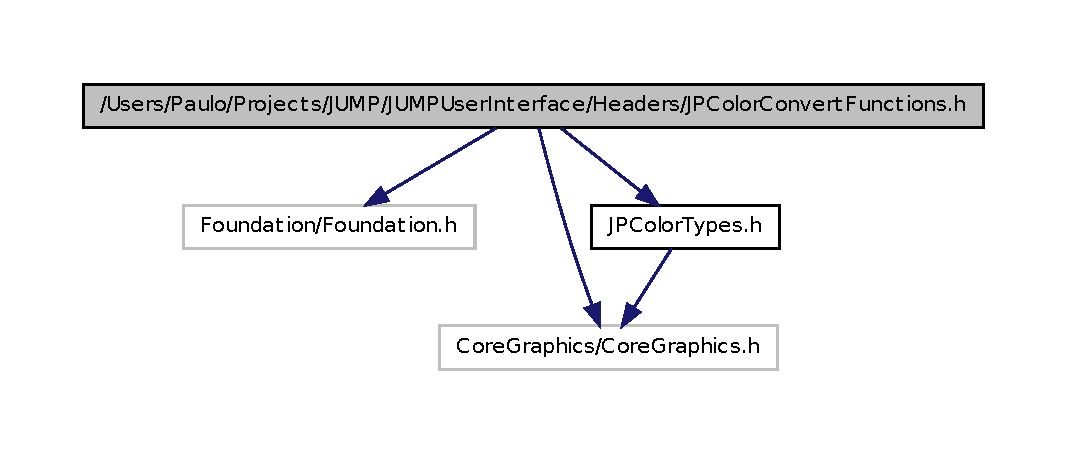
\includegraphics[width=400pt]{_j_p_color_convert_functions_8h__incl}
\end{center}
\end{figure}
This graph shows which files directly or indirectly include this file:\nopagebreak
\begin{figure}[H]
\begin{center}
\leavevmode
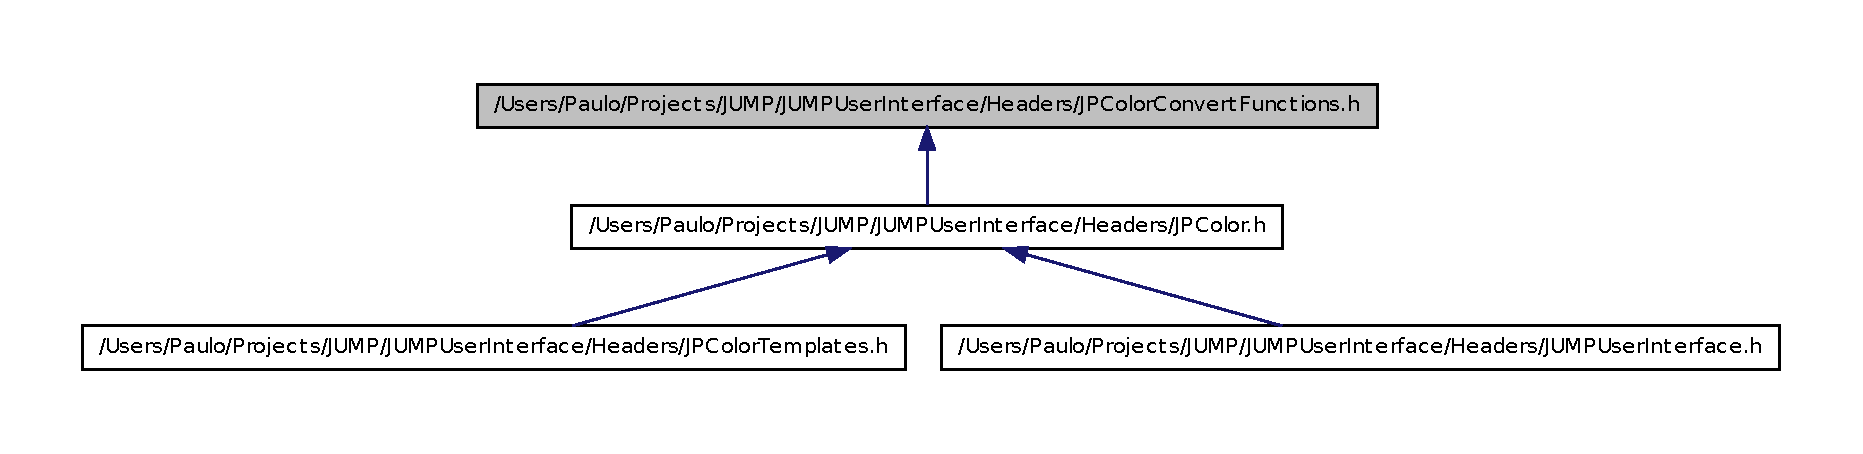
\includegraphics[width=400pt]{_j_p_color_convert_functions_8h__dep__incl}
\end{center}
\end{figure}
\subsection*{Functions}
\begin{DoxyCompactItemize}
\item 
\hypertarget{_j_p_color_convert_functions_8h_a8c9831bc0a46f817ca27293ee2c3136d}{
\hyperlink{struct_j_pcmyk}{JPcmyk} \hyperlink{_j_p_color_convert_functions_8h_a8c9831bc0a46f817ca27293ee2c3136d}{JPConvertRGBtoCMYK} (\hyperlink{struct_j_prgb}{JPrgb} RGB)}
\label{_j_p_color_convert_functions_8h_a8c9831bc0a46f817ca27293ee2c3136d}

\begin{DoxyCompactList}\small\item\em Convert from RGB to CMYK. \item\end{DoxyCompactList}\item 
\hypertarget{_j_p_color_convert_functions_8h_afbace75877e5f8a1e13cd3cd6862d5dc}{
\hyperlink{struct_j_prgb}{JPrgb} \hyperlink{_j_p_color_convert_functions_8h_afbace75877e5f8a1e13cd3cd6862d5dc}{JPConvertCMYKtoRGB} (\hyperlink{struct_j_pcmyk}{JPcmyk} CMYK)}
\label{_j_p_color_convert_functions_8h_afbace75877e5f8a1e13cd3cd6862d5dc}

\begin{DoxyCompactList}\small\item\em Convert from CMYK to RGB. \item\end{DoxyCompactList}\item 
\hypertarget{_j_p_color_convert_functions_8h_ab9d9002d48aff333c31d3b5c30512648}{
\hyperlink{struct_j_phsv}{JPhsv} \hyperlink{_j_p_color_convert_functions_8h_ab9d9002d48aff333c31d3b5c30512648}{JPConvertRGBtoHSV} (\hyperlink{struct_j_prgb}{JPrgb} RGB)}
\label{_j_p_color_convert_functions_8h_ab9d9002d48aff333c31d3b5c30512648}

\begin{DoxyCompactList}\small\item\em Convert from RGB to HSV. \item\end{DoxyCompactList}\item 
\hypertarget{_j_p_color_convert_functions_8h_a5dc60c232611ea3801fa48d1b77dc9f7}{
\hyperlink{struct_j_prgb}{JPrgb} \hyperlink{_j_p_color_convert_functions_8h_a5dc60c232611ea3801fa48d1b77dc9f7}{JPConvertHSVtoRGB} (\hyperlink{struct_j_phsv}{JPhsv} HSB)}
\label{_j_p_color_convert_functions_8h_a5dc60c232611ea3801fa48d1b77dc9f7}

\begin{DoxyCompactList}\small\item\em Convert from HSV to RGB. \item\end{DoxyCompactList}\item 
\hypertarget{_j_p_color_convert_functions_8h_a29fb68443cbbf65e6156359c7cb1627e}{
\hyperlink{struct_j_pxyz}{JPxyz} \hyperlink{_j_p_color_convert_functions_8h_a29fb68443cbbf65e6156359c7cb1627e}{JPConvertRGBtoXYZ} (\hyperlink{struct_j_prgb}{JPrgb} RGB)}
\label{_j_p_color_convert_functions_8h_a29fb68443cbbf65e6156359c7cb1627e}

\begin{DoxyCompactList}\small\item\em Convert from RGB to XYZ. \item\end{DoxyCompactList}\item 
\hypertarget{_j_p_color_convert_functions_8h_ae899918e8be7891c163413db268fdbab}{
\hyperlink{struct_j_prgb}{JPrgb} \hyperlink{_j_p_color_convert_functions_8h_ae899918e8be7891c163413db268fdbab}{JPConvertHSBtoXYZ} (\hyperlink{struct_j_pxyz}{JPxyz} XYZ)}
\label{_j_p_color_convert_functions_8h_ae899918e8be7891c163413db268fdbab}

\begin{DoxyCompactList}\small\item\em Convert from HSV to RGB. \item\end{DoxyCompactList}\item 
\hypertarget{_j_p_color_convert_functions_8h_a6accfe9bd47d3c1f3eb4b44fec5ff353}{
\hyperlink{struct_j_plab}{JPlab} \hyperlink{_j_p_color_convert_functions_8h_a6accfe9bd47d3c1f3eb4b44fec5ff353}{JPConvertRGBtoLAB} (\hyperlink{struct_j_prgb}{JPrgb} RGB)}
\label{_j_p_color_convert_functions_8h_a6accfe9bd47d3c1f3eb4b44fec5ff353}

\begin{DoxyCompactList}\small\item\em Convert from RGB to LAB. \item\end{DoxyCompactList}\item 
\hypertarget{_j_p_color_convert_functions_8h_a5c87e958f95fbb67624408d65d72857b}{
\hyperlink{struct_j_prgb}{JPrgb} \hyperlink{_j_p_color_convert_functions_8h_a5c87e958f95fbb67624408d65d72857b}{JPConvertLABtoRGB} (\hyperlink{struct_j_plab}{JPlab} LAB)}
\label{_j_p_color_convert_functions_8h_a5c87e958f95fbb67624408d65d72857b}

\begin{DoxyCompactList}\small\item\em Convert from LAB to RGB. \item\end{DoxyCompactList}\item 
\hypertarget{_j_p_color_convert_functions_8h_a057f954c411c5a945805fa936f5e65ee}{
\hyperlink{struct_j_plab}{JPlab} \hyperlink{_j_p_color_convert_functions_8h_a057f954c411c5a945805fa936f5e65ee}{JPConvertXYZtoLAB} (\hyperlink{struct_j_pxyz}{JPxyz} XYZ)}
\label{_j_p_color_convert_functions_8h_a057f954c411c5a945805fa936f5e65ee}

\begin{DoxyCompactList}\small\item\em Convert from XYZ to LAB. \item\end{DoxyCompactList}\item 
\hypertarget{_j_p_color_convert_functions_8h_a488927881de1236b0531c11a980c8167}{
\hyperlink{struct_j_pxyz}{JPxyz} \hyperlink{_j_p_color_convert_functions_8h_a488927881de1236b0531c11a980c8167}{JPConvertLABtoXYZ} (\hyperlink{struct_j_plab}{JPlab} LAB)}
\label{_j_p_color_convert_functions_8h_a488927881de1236b0531c11a980c8167}

\begin{DoxyCompactList}\small\item\em Convert from LAB to XYZ. \item\end{DoxyCompactList}\item 
\hypertarget{_j_p_color_convert_functions_8h_a9550049a164deabf38a82f59a230a431}{
\hyperlink{struct_j_prgb}{JPrgb} \hyperlink{_j_p_color_convert_functions_8h_a9550049a164deabf38a82f59a230a431}{JPConvertXYZtoRGB} (\hyperlink{struct_j_pxyz}{JPxyz} XYZ)}
\label{_j_p_color_convert_functions_8h_a9550049a164deabf38a82f59a230a431}

\begin{DoxyCompactList}\small\item\em Convert from XYZ to RGB. \item\end{DoxyCompactList}\end{DoxyCompactItemize}


\subsection{Detailed Description}
\hyperlink{interface_j_p_color}{JPColor} functions to convert between color spaces. 
\hypertarget{_j_p_color_functions_8h}{
\section{/Users/Paulo/Projects/JUMP/JUMPUserInterface/Headers/JPColorFunctions.h File Reference}
\label{_j_p_color_functions_8h}\index{/Users/Paulo/Projects/JUMP/JUMPUserInterface/Headers/JPColorFunctions.h@{/Users/Paulo/Projects/JUMP/JUMPUserInterface/Headers/JPColorFunctions.h}}
}


\hyperlink{interface_j_p_color}{JPColor} utility and helper functions.  


{\ttfamily \#import \char`\"{}JPColorTypes.h\char`\"{}}\par
{\ttfamily \#import $<$Foundation/Foundation.h$>$}\par
{\ttfamily \#import $<$CoreGraphics/CoreGraphics.h$>$}\par
Include dependency graph for JPColorFunctions.h:\nopagebreak
\begin{figure}[H]
\begin{center}
\leavevmode
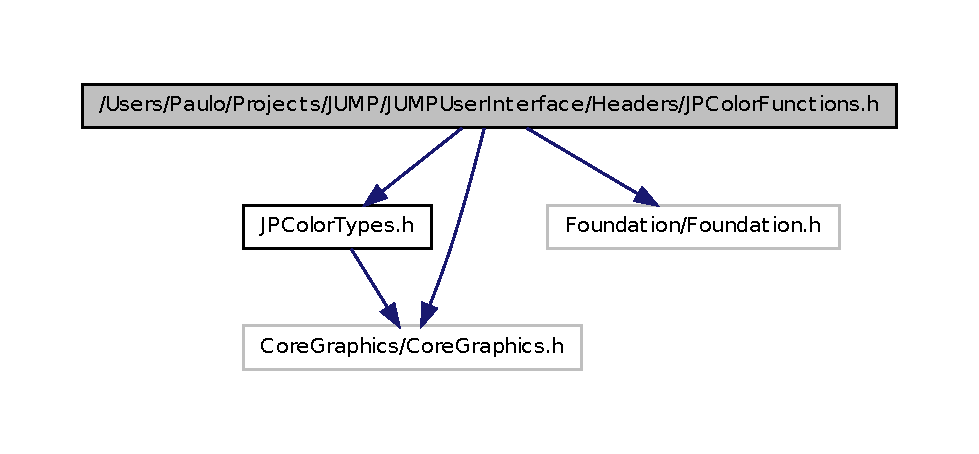
\includegraphics[width=400pt]{_j_p_color_functions_8h__incl}
\end{center}
\end{figure}
This graph shows which files directly or indirectly include this file:\nopagebreak
\begin{figure}[H]
\begin{center}
\leavevmode
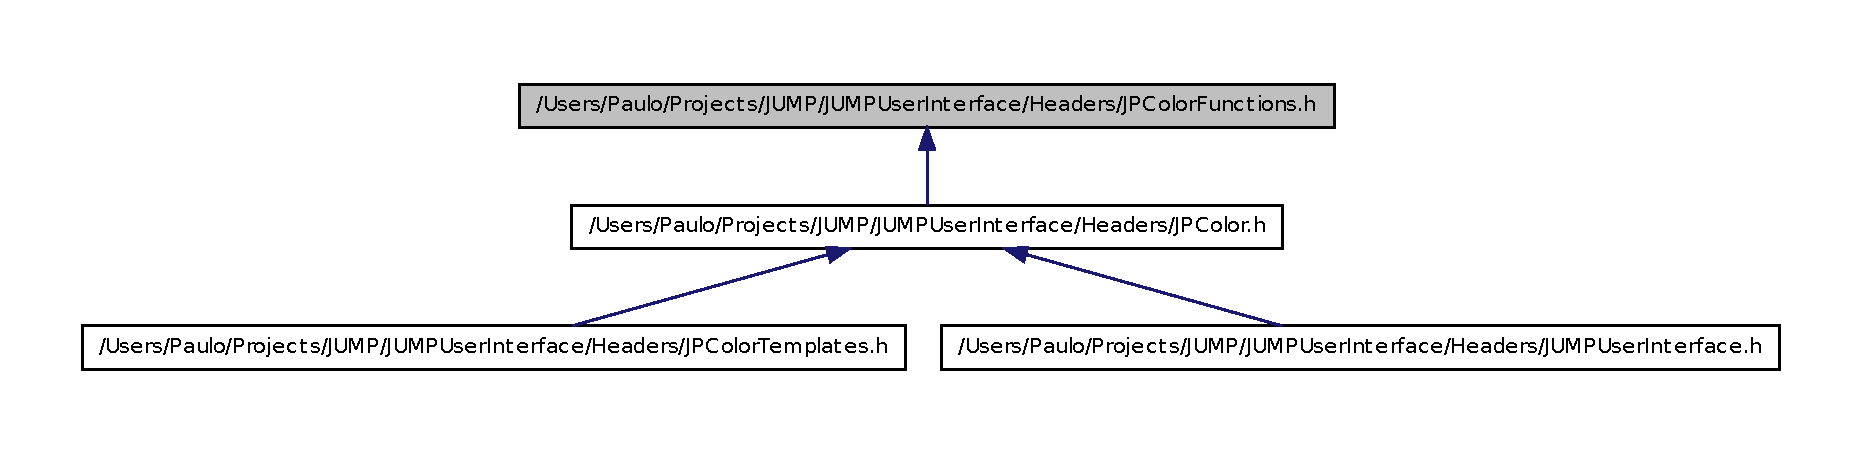
\includegraphics[width=400pt]{_j_p_color_functions_8h__dep__incl}
\end{center}
\end{figure}
\subsection*{Defines}
\begin{DoxyCompactItemize}
\item 
\hypertarget{_j_p_color_functions_8h_a41c757dadd61fafc580a4ac21b2c34de}{
\#define \hyperlink{_j_p_color_functions_8h_a41c757dadd61fafc580a4ac21b2c34de}{JPConvertAlpha}(alpha)~( (float)alpha / 100.0 )}
\label{_j_p_color_functions_8h_a41c757dadd61fafc580a4ac21b2c34de}

\begin{DoxyCompactList}\small\item\em Convert a Quartz Alpha Percent (0.0 -\/ 1.0) to Photoshop-\/like Alpha Percent (0 -\/ 100). \item\end{DoxyCompactList}\item 
\hypertarget{_j_p_color_functions_8h_a57bdba7b6ff34e900244d883d5ef8e92}{
\#define \hyperlink{_j_p_color_functions_8h_a57bdba7b6ff34e900244d883d5ef8e92}{JPPSToQuartz}(color)~(float)( color / 255.0 )}
\label{_j_p_color_functions_8h_a57bdba7b6ff34e900244d883d5ef8e92}

\begin{DoxyCompactList}\small\item\em Convert a Photoshop Color Percent (0 -\/ 255) to a Quartz Color Percent (0.0 -\/ 1.0). \item\end{DoxyCompactList}\item 
\hypertarget{_j_p_color_functions_8h_ac8bcc1fdbf3dfe6c27084df45a42e8b7}{
\#define \hyperlink{_j_p_color_functions_8h_ac8bcc1fdbf3dfe6c27084df45a42e8b7}{JPQuartzToPS}(\_\-\_\-color\_\-\_\-)~(int)roundf( \_\-\_\-color\_\-\_\-  $\ast$ 255 )}
\label{_j_p_color_functions_8h_ac8bcc1fdbf3dfe6c27084df45a42e8b7}

\begin{DoxyCompactList}\small\item\em Convert a Quartz Color Percent (0.0 -\/ 1.0) to a Photoshop-\/like Color Percent (0 -\/ 255). \item\end{DoxyCompactList}\item 
\hypertarget{_j_p_color_functions_8h_a279f0819120931b0413f5fcb2e3e8c04}{
\#define \hyperlink{_j_p_color_functions_8h_a279f0819120931b0413f5fcb2e3e8c04}{JPCreateUIColor}(r, g, b, alpha)~( \mbox{[}UIColor colorWithCGColor:JPCreateRGBColor( (float)r, (float)g, (float)b, (float)alpha) \mbox{]}  )}
\label{_j_p_color_functions_8h_a279f0819120931b0413f5fcb2e3e8c04}

\begin{DoxyCompactList}\small\item\em Return a UIColor based on a Photoshop Color Percent (0 -\/ 255) for Red, Green and Blue. \item\end{DoxyCompactList}\item 
\hypertarget{_j_p_color_functions_8h_ad3b58eeaceba397fc605d21b8f9a0c41}{
\#define \hyperlink{_j_p_color_functions_8h_ad3b58eeaceba397fc605d21b8f9a0c41}{JPNormalizeUp}(color)~((int)roundf( color $\ast$ 100 ))}
\label{_j_p_color_functions_8h_ad3b58eeaceba397fc605d21b8f9a0c41}

\begin{DoxyCompactList}\small\item\em Normalize some value to 0-\/1;. \item\end{DoxyCompactList}\item 
\hypertarget{_j_p_color_functions_8h_aba20205288ce7f0cdb7618aa6af36e8a}{
\#define \hyperlink{_j_p_color_functions_8h_aba20205288ce7f0cdb7618aa6af36e8a}{JPNormalizeDown}(\_\-\_\-color\_\-\_\-)~((float)\_\-\_\-color\_\-\_\- / 100)}
\label{_j_p_color_functions_8h_aba20205288ce7f0cdb7618aa6af36e8a}

\begin{DoxyCompactList}\small\item\em Normalize some value to 0-\/100;. \item\end{DoxyCompactList}\end{DoxyCompactItemize}
\subsection*{Functions}
\begin{DoxyCompactItemize}
\item 
CGColorRef \hyperlink{_j_p_color_functions_8h_a4a5f10912287a18d4d079db2473f1e5a}{JPCreateRGBColor} (float r, float g, float b, float alpha)
\begin{DoxyCompactList}\small\item\em Create a Quartz CGColor based on a Photoshop-\/like Color Percent (0 -\/ 255) for Red, Green and Blue. \item\end{DoxyCompactList}\item 
CGColorRef \hyperlink{_j_p_color_functions_8h_adfd936f6725e5d8047fb95fbb0882e4b}{JPCreateColorWithJPrgb} (\hyperlink{struct_j_prgb}{JPrgb} RGB, float alpha)
\begin{DoxyCompactList}\small\item\em Create a Quartz CGColor based on a \hyperlink{struct_j_prgb}{JPrgb} Type. \item\end{DoxyCompactList}\item 
\hypertarget{_j_p_color_functions_8h_a1eda119ff0f5566f886a81a784c67388}{
\hyperlink{struct_j_prgb}{JPrgb} \hyperlink{_j_p_color_functions_8h_a1eda119ff0f5566f886a81a784c67388}{JPCreateRGBType} (int r, int g, int b)}
\label{_j_p_color_functions_8h_a1eda119ff0f5566f886a81a784c67388}

\begin{DoxyCompactList}\small\item\em Create an \hyperlink{struct_j_prgb}{JPrgb} structure type. \item\end{DoxyCompactList}\item 
\hypertarget{_j_p_color_functions_8h_ace4eb5bbf6392366d0cc6ae57313d6d8}{
\hyperlink{struct_j_pcmyk}{JPcmyk} \hyperlink{_j_p_color_functions_8h_ace4eb5bbf6392366d0cc6ae57313d6d8}{JPCreateCMYKType} (int C, int M, int Y, int K)}
\label{_j_p_color_functions_8h_ace4eb5bbf6392366d0cc6ae57313d6d8}

\begin{DoxyCompactList}\small\item\em Create an \hyperlink{struct_j_pcmyk}{JPcmyk} structure type. \item\end{DoxyCompactList}\item 
\hypertarget{_j_p_color_functions_8h_ab10ba17e60d2703b7cd09c7737467062}{
\hyperlink{struct_j_plab}{JPlab} \hyperlink{_j_p_color_functions_8h_ab10ba17e60d2703b7cd09c7737467062}{JPCreateLABType} (int L, int A, int B)}
\label{_j_p_color_functions_8h_ab10ba17e60d2703b7cd09c7737467062}

\begin{DoxyCompactList}\small\item\em Create an \hyperlink{struct_j_plab}{JPlab} structure type. \item\end{DoxyCompactList}\item 
\hypertarget{_j_p_color_functions_8h_ac6031c5fd2d719a6b618d030c86cc6ac}{
\hyperlink{struct_j_phsv}{JPhsv} \hyperlink{_j_p_color_functions_8h_ac6031c5fd2d719a6b618d030c86cc6ac}{JPCreateHSVType} (int H, int S, int B)}
\label{_j_p_color_functions_8h_ac6031c5fd2d719a6b618d030c86cc6ac}

\begin{DoxyCompactList}\small\item\em Create an \hyperlink{struct_j_phsv}{JPhsv} structure type. \item\end{DoxyCompactList}\end{DoxyCompactItemize}


\subsection{Detailed Description}
\hyperlink{interface_j_p_color}{JPColor} utility and helper functions. 

\subsection{Function Documentation}
\hypertarget{_j_p_color_functions_8h_a4a5f10912287a18d4d079db2473f1e5a}{
\index{JPColorFunctions.h@{JPColorFunctions.h}!JPCreateRGBColor@{JPCreateRGBColor}}
\index{JPCreateRGBColor@{JPCreateRGBColor}!JPColorFunctions.h@{JPColorFunctions.h}}
\subsubsection[{JPCreateRGBColor}]{\setlength{\rightskip}{0pt plus 5cm}CGColorRef JPCreateRGBColor (
\begin{DoxyParamCaption}
\item[{float}]{r, }
\item[{float}]{g, }
\item[{float}]{b, }
\item[{float}]{alpha}
\end{DoxyParamCaption}
)}}
\label{_j_p_color_functions_8h_a4a5f10912287a18d4d079db2473f1e5a}


Create a Quartz CGColor based on a Photoshop-\/like Color Percent (0 -\/ 255) for Red, Green and Blue. 


\begin{DoxyParams}{Parameters}
{\em r} & An Red value from 0 to 255. \\
\hline
{\em g} & An Green value from 0 to 255. \\
\hline
{\em b} & An Blue value from 0 to 255. \\
\hline
{\em alpha} & An opacity value from 0 to 100. \\
\hline
\end{DoxyParams}
\begin{DoxyReturn}{Returns}
An retained Quartz CGColorRef object. 
\end{DoxyReturn}
\hypertarget{_j_p_color_functions_8h_adfd936f6725e5d8047fb95fbb0882e4b}{
\index{JPColorFunctions.h@{JPColorFunctions.h}!JPCreateColorWithJPrgb@{JPCreateColorWithJPrgb}}
\index{JPCreateColorWithJPrgb@{JPCreateColorWithJPrgb}!JPColorFunctions.h@{JPColorFunctions.h}}
\subsubsection[{JPCreateColorWithJPrgb}]{\setlength{\rightskip}{0pt plus 5cm}CGColorRef JPCreateColorWithJPrgb (
\begin{DoxyParamCaption}
\item[{{\bf JPrgb}}]{RGB, }
\item[{float}]{alpha}
\end{DoxyParamCaption}
)}}
\label{_j_p_color_functions_8h_adfd936f6725e5d8047fb95fbb0882e4b}


Create a Quartz CGColor based on a \hyperlink{struct_j_prgb}{JPrgb} Type. 


\begin{DoxyParams}{Parameters}
{\em RGB} & An \hyperlink{struct_j_prgb}{JPrgb} type with values. \\
\hline
{\em alpha} & An opacity value from 0 to 100. \\
\hline
\end{DoxyParams}
\begin{DoxyReturn}{Returns}
An retained Quartz CGColorRef object. 
\end{DoxyReturn}

\hypertarget{_j_p_color_types_8h}{
\section{/Users/Paulo/Projects/JUMP/JUMPUserInterface/Headers/JPColorTypes.h File Reference}
\label{_j_p_color_types_8h}\index{/Users/Paulo/Projects/JUMP/JUMPUserInterface/Headers/JPColorTypes.h@{/Users/Paulo/Projects/JUMP/JUMPUserInterface/Headers/JPColorTypes.h}}
}


\hyperlink{interface_j_p_color}{JPColor} Data Type Structure for different color spaces.  


{\ttfamily \#import $<$CoreGraphics/CoreGraphics.h$>$}\par
Include dependency graph for JPColorTypes.h:\nopagebreak
\begin{figure}[H]
\begin{center}
\leavevmode
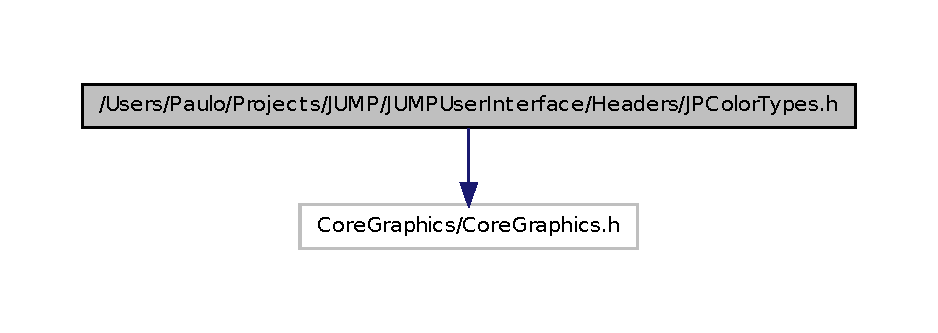
\includegraphics[width=400pt]{_j_p_color_types_8h__incl}
\end{center}
\end{figure}
This graph shows which files directly or indirectly include this file:\nopagebreak
\begin{figure}[H]
\begin{center}
\leavevmode
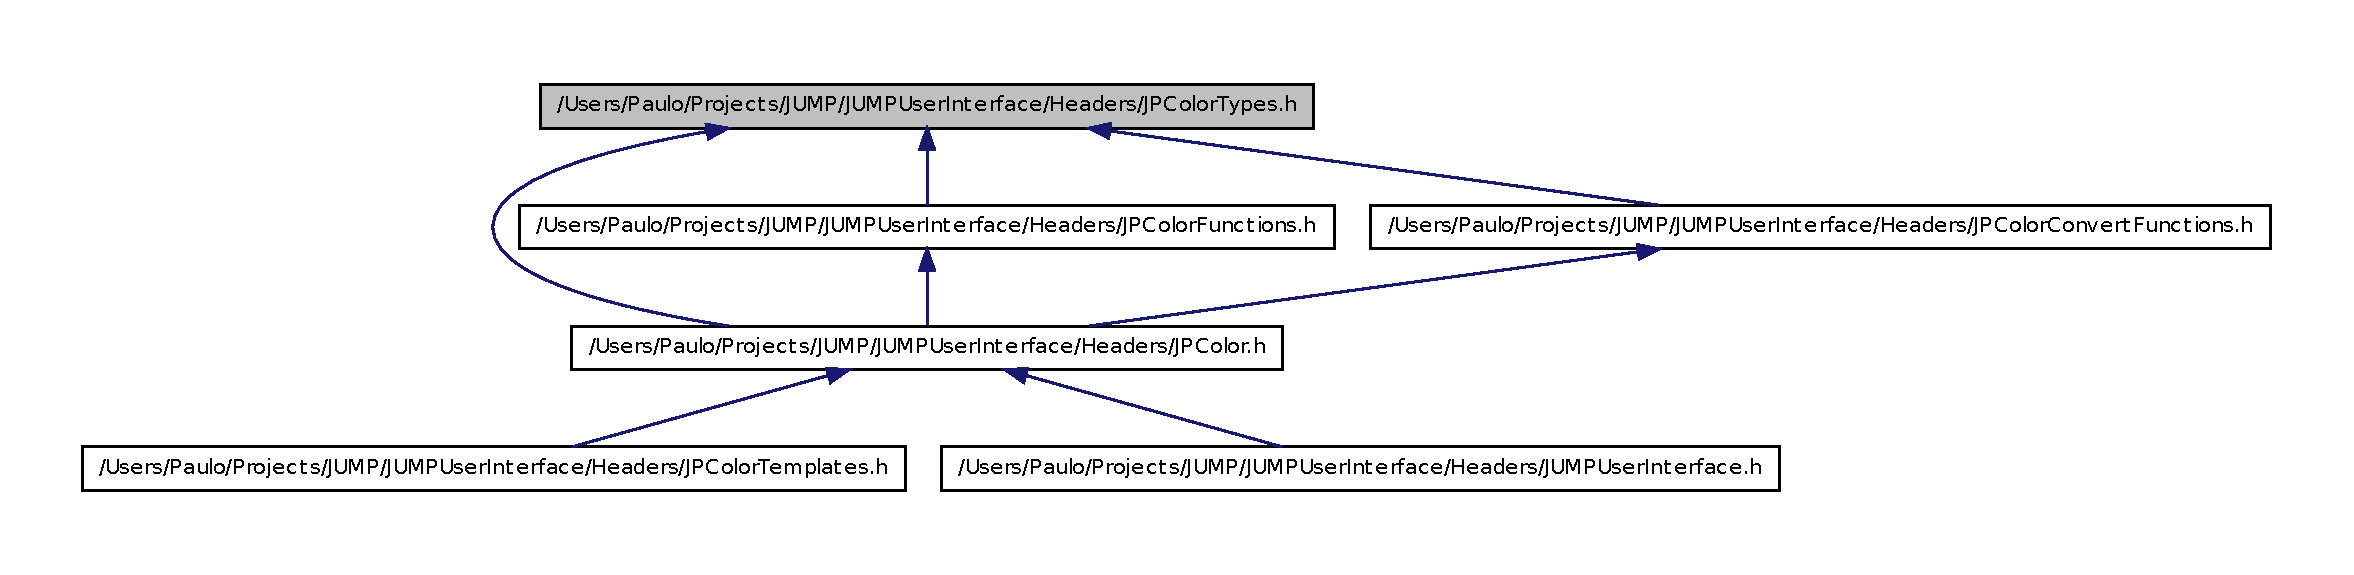
\includegraphics[width=400pt]{_j_p_color_types_8h__dep__incl}
\end{center}
\end{figure}
\subsection*{Classes}
\begin{DoxyCompactItemize}
\item 
struct \hyperlink{struct_j_prgb}{JPrgb}
\begin{DoxyCompactList}\small\item\em \hyperlink{interface_j_p_color}{JPColor} RGB Structure Type. \item\end{DoxyCompactList}\item 
struct \hyperlink{struct_j_pcmy}{JPcmy}
\begin{DoxyCompactList}\small\item\em \hyperlink{interface_j_p_color}{JPColor} CMY Structure Type. \item\end{DoxyCompactList}\item 
struct \hyperlink{struct_j_pcmyk}{JPcmyk}
\begin{DoxyCompactList}\small\item\em \hyperlink{interface_j_p_color}{JPColor} CMYK Structure Type. \item\end{DoxyCompactList}\item 
struct \hyperlink{struct_j_phsv}{JPhsv}
\begin{DoxyCompactList}\small\item\em \hyperlink{interface_j_p_color}{JPColor} HSB Structure Type. \item\end{DoxyCompactList}\item 
struct \hyperlink{struct_j_plab}{JPlab}
\begin{DoxyCompactList}\small\item\em \hyperlink{interface_j_p_color}{JPColor} LAB Structure Type. Use \hyperlink{_j_p_color_functions_8h_ab10ba17e60d2703b7cd09c7737467062}{JPCreateLABType} to conveniently create this structure. \item\end{DoxyCompactList}\item 
struct \hyperlink{struct_j_pxyz}{JPxyz}
\begin{DoxyCompactList}\small\item\em \hyperlink{interface_j_p_color}{JPColor} XYZ Structure Type. \item\end{DoxyCompactList}\end{DoxyCompactItemize}


\subsection{Detailed Description}
\hyperlink{interface_j_p_color}{JPColor} Data Type Structure for different color spaces. 
\printindex
\end{document}
